% Options for packages loaded elsewhere
\PassOptionsToPackage{unicode}{hyperref}
\PassOptionsToPackage{hyphens}{url}
%
\documentclass[
  10pt,
  b5paper,
  oneside]{book}
\usepackage{amsmath,amssymb}
\usepackage{lmodern}
\usepackage{iftex}
\ifPDFTeX
  \usepackage[T1]{fontenc}
  \usepackage[utf8]{inputenc}
  \usepackage{textcomp} % provide euro and other symbols
\else % if luatex or xetex
  \usepackage{unicode-math}
  \defaultfontfeatures{Scale=MatchLowercase}
  \defaultfontfeatures[\rmfamily]{Ligatures=TeX,Scale=1}
\fi
% Use upquote if available, for straight quotes in verbatim environments
\IfFileExists{upquote.sty}{\usepackage{upquote}}{}
\IfFileExists{microtype.sty}{% use microtype if available
  \usepackage[]{microtype}
  \UseMicrotypeSet[protrusion]{basicmath} % disable protrusion for tt fonts
}{}
\makeatletter
\@ifundefined{KOMAClassName}{% if non-KOMA class
  \IfFileExists{parskip.sty}{%
    \usepackage{parskip}
  }{% else
    \setlength{\parindent}{0pt}
    \setlength{\parskip}{6pt plus 2pt minus 1pt}}
}{% if KOMA class
  \KOMAoptions{parskip=half}}
\makeatother
\usepackage{xcolor}
\usepackage{color}
\usepackage{fancyvrb}
\newcommand{\VerbBar}{|}
\newcommand{\VERB}{\Verb[commandchars=\\\{\}]}
\DefineVerbatimEnvironment{Highlighting}{Verbatim}{commandchars=\\\{\}}
% Add ',fontsize=\small' for more characters per line
\usepackage{framed}
\definecolor{shadecolor}{RGB}{248,248,248}
\newenvironment{Shaded}{\begin{snugshade}}{\end{snugshade}}
\newcommand{\AlertTok}[1]{\textcolor[rgb]{0.94,0.16,0.16}{#1}}
\newcommand{\AnnotationTok}[1]{\textcolor[rgb]{0.56,0.35,0.01}{\textbf{\textit{#1}}}}
\newcommand{\AttributeTok}[1]{\textcolor[rgb]{0.77,0.63,0.00}{#1}}
\newcommand{\BaseNTok}[1]{\textcolor[rgb]{0.00,0.00,0.81}{#1}}
\newcommand{\BuiltInTok}[1]{#1}
\newcommand{\CharTok}[1]{\textcolor[rgb]{0.31,0.60,0.02}{#1}}
\newcommand{\CommentTok}[1]{\textcolor[rgb]{0.56,0.35,0.01}{\textit{#1}}}
\newcommand{\CommentVarTok}[1]{\textcolor[rgb]{0.56,0.35,0.01}{\textbf{\textit{#1}}}}
\newcommand{\ConstantTok}[1]{\textcolor[rgb]{0.00,0.00,0.00}{#1}}
\newcommand{\ControlFlowTok}[1]{\textcolor[rgb]{0.13,0.29,0.53}{\textbf{#1}}}
\newcommand{\DataTypeTok}[1]{\textcolor[rgb]{0.13,0.29,0.53}{#1}}
\newcommand{\DecValTok}[1]{\textcolor[rgb]{0.00,0.00,0.81}{#1}}
\newcommand{\DocumentationTok}[1]{\textcolor[rgb]{0.56,0.35,0.01}{\textbf{\textit{#1}}}}
\newcommand{\ErrorTok}[1]{\textcolor[rgb]{0.64,0.00,0.00}{\textbf{#1}}}
\newcommand{\ExtensionTok}[1]{#1}
\newcommand{\FloatTok}[1]{\textcolor[rgb]{0.00,0.00,0.81}{#1}}
\newcommand{\FunctionTok}[1]{\textcolor[rgb]{0.00,0.00,0.00}{#1}}
\newcommand{\ImportTok}[1]{#1}
\newcommand{\InformationTok}[1]{\textcolor[rgb]{0.56,0.35,0.01}{\textbf{\textit{#1}}}}
\newcommand{\KeywordTok}[1]{\textcolor[rgb]{0.13,0.29,0.53}{\textbf{#1}}}
\newcommand{\NormalTok}[1]{#1}
\newcommand{\OperatorTok}[1]{\textcolor[rgb]{0.81,0.36,0.00}{\textbf{#1}}}
\newcommand{\OtherTok}[1]{\textcolor[rgb]{0.56,0.35,0.01}{#1}}
\newcommand{\PreprocessorTok}[1]{\textcolor[rgb]{0.56,0.35,0.01}{\textit{#1}}}
\newcommand{\RegionMarkerTok}[1]{#1}
\newcommand{\SpecialCharTok}[1]{\textcolor[rgb]{0.00,0.00,0.00}{#1}}
\newcommand{\SpecialStringTok}[1]{\textcolor[rgb]{0.31,0.60,0.02}{#1}}
\newcommand{\StringTok}[1]{\textcolor[rgb]{0.31,0.60,0.02}{#1}}
\newcommand{\VariableTok}[1]{\textcolor[rgb]{0.00,0.00,0.00}{#1}}
\newcommand{\VerbatimStringTok}[1]{\textcolor[rgb]{0.31,0.60,0.02}{#1}}
\newcommand{\WarningTok}[1]{\textcolor[rgb]{0.56,0.35,0.01}{\textbf{\textit{#1}}}}
\usepackage{longtable,booktabs,array}
\usepackage{calc} % for calculating minipage widths
% Correct order of tables after \paragraph or \subparagraph
\usepackage{etoolbox}
\makeatletter
\patchcmd\longtable{\par}{\if@noskipsec\mbox{}\fi\par}{}{}
\makeatother
% Allow footnotes in longtable head/foot
\IfFileExists{footnotehyper.sty}{\usepackage{footnotehyper}}{\usepackage{footnote}}
\makesavenoteenv{longtable}
\usepackage{graphicx}
\makeatletter
\def\maxwidth{\ifdim\Gin@nat@width>\linewidth\linewidth\else\Gin@nat@width\fi}
\def\maxheight{\ifdim\Gin@nat@height>\textheight\textheight\else\Gin@nat@height\fi}
\makeatother
% Scale images if necessary, so that they will not overflow the page
% margins by default, and it is still possible to overwrite the defaults
% using explicit options in \includegraphics[width, height, ...]{}
\setkeys{Gin}{width=\maxwidth,height=\maxheight,keepaspectratio}
% Set default figure placement to htbp
\makeatletter
\def\fps@figure{htbp}
\makeatother
\setlength{\emergencystretch}{3em} % prevent overfull lines
\providecommand{\tightlist}{%
  \setlength{\itemsep}{0pt}\setlength{\parskip}{0pt}}
\setcounter{secnumdepth}{5}
\newlength{\cslhangindent}
\setlength{\cslhangindent}{1.5em}
\newlength{\csllabelwidth}
\setlength{\csllabelwidth}{3em}
\newlength{\cslentryspacingunit} % times entry-spacing
\setlength{\cslentryspacingunit}{\parskip}
\newenvironment{CSLReferences}[2] % #1 hanging-ident, #2 entry spacing
 {% don't indent paragraphs
  \setlength{\parindent}{0pt}
  % turn on hanging indent if param 1 is 1
  \ifodd #1
  \let\oldpar\par
  \def\par{\hangindent=\cslhangindent\oldpar}
  \fi
  % set entry spacing
  \setlength{\parskip}{#2\cslentryspacingunit}
 }%
 {}
\usepackage{calc}
\newcommand{\CSLBlock}[1]{#1\hfill\break}
\newcommand{\CSLLeftMargin}[1]{\parbox[t]{\csllabelwidth}{#1}}
\newcommand{\CSLRightInline}[1]{\parbox[t]{\linewidth - \csllabelwidth}{#1}\break}
\newcommand{\CSLIndent}[1]{\hspace{\cslhangindent}#1}
\AtBeginDocument{\renewcommand{\chaptername}{Chapter}}
\usepackage{titling}
\usepackage{natbib}
\usepackage{pdfpages}
\usepackage{fancyhdr}
\usepackage{booktabs}
\usepackage{longtable}
\usepackage{subfig}
\usepackage{array}
\usepackage{amsmath}
\usepackage{multirow}
\usepackage{wrapfig}
\usepackage{bookmark}
\usepackage[utf8]{inputenc}
\usepackage{float}
\usepackage{colortbl}
\usepackage{pdflscape}
\usepackage{tabu}
\usepackage{threeparttable}
\usepackage{threeparttablex}
\usepackage[normalem]{ulem}
\usepackage{makecell}
\usepackage{xcolor}
\DeclareUnicodeCharacter{2212}{\textendash}
\usepackage{rotating, graphicx}
\usepackage{listings}
\ifLuaTeX
  \usepackage{selnolig}  % disable illegal ligatures
\fi
\IfFileExists{bookmark.sty}{\usepackage{bookmark}}{\usepackage{hyperref}}
\IfFileExists{xurl.sty}{\usepackage{xurl}}{} % add URL line breaks if available
\urlstyle{same} % disable monospaced font for URLs
\hypersetup{
  pdftitle={ Soil Sampling Design},
  pdfauthor={Rodríguez Lado, L., Angelini, M.E, Naypewe, N., Luotto, I., Yigini, Y.},
  hidelinks,
  pdfcreator={LaTeX via pandoc}}

\title{
Soil Sampling Design}
\usepackage{etoolbox}
\makeatletter
\providecommand{\subtitle}[1]{% add subtitle to \maketitle
  \apptocmd{\@title}{\par {\large #1 \par}}{}{}
}
\makeatother
\subtitle{Technical Manual}
\author{Rodríguez Lado, L., Angelini, M.E, Naypewe, N., Luotto, I., Yigini, Y.}
\date{2023-12-22}

\begin{document}
\maketitle

{
\setcounter{tocdepth}{1}
\tableofcontents
}
\frontmatter
\addtocontents{toc}{\protect\hypersetup{hidelinks}}   
\addtocontents{lof}{\protect\hypersetup{hidelinks}}
\addtocontents{lot}{\protect\hypersetup{hidelinks}}
\addtocontents{lot}{\protect\hypersetup{hidelinks}}
\addtocontents{lot}{\protect\hypersetup{hidelinks}}
\tableofcontents
\listoffigures
\listoftables
\nopagebreak[5]

\begin{figure}

\includegraphics[width=34.46in]{images/frontcover} \end{figure}

\hypertarget{licence}{%
\chapter*{Licence}\label{licence}}
\addcontentsline{toc}{chapter}{Licence}

The GSNmap Technical Manual is made available under the Creative Commons Attribution-NonCommercial-ShareAlike 3.0 IGO licence

\href{https://creativecommons.org/licenses/by-nc-sa/3.0/igo/legalcode}{CC BY-NC-SA 3.0 IGO}.

\hypertarget{abbreviations-and-acronyms}{%
\chapter*{Abbreviations and acronyms}\label{abbreviations-and-acronyms}}
\addcontentsline{toc}{chapter}{Abbreviations and acronyms}

\begin{description}
\item[BD]
Bulk density
\item[CEC]
Cation exchange capacity
\item[CRAN]
Comprehensive R archive network
\end{description}

\hypertarget{contributors-and-reviewers}{%
\chapter*{Contributors and reviewers}\label{contributors-and-reviewers}}
\addcontentsline{toc}{chapter}{Contributors and reviewers}

\textbf{International Network of Soil Information Institutions}\\

\textbf{GSP - Soil Information and Data}\\

\hypertarget{introduction}{%
\chapter{Introduction}\label{introduction}}

The success of soil mapping activities relies on the existence of proper data collated through detailed soil sampling protocols ensuring representative and reliable soil data collection. This publication does not intend to be an intensive compilation which cover all the intricate possibilities in soil sampling design. In turn, we show a number of different soil sampling protocols through examples, covering both the most common approaches that can be used for the design of field soil sampling and present methodologies to evaluate their accuracy and effectiveness. The last part of the manual is particularly focused in the use of conditional Latin Hypercube Sampling (cLHS), a statistical methodology developed specifically for soil sampling from a Digital Soil Mapping perspective (\protect\hyperlink{ref-minasny2006}{Minasny and McBratney, 2006}).

The manual is structured in two parts. \texttt{\textquotesingle{}Part\ One\textquotesingle{}} presents a methodology to evaluate the capacity of an existing soil legacy data to represent the potential soil diversity within a certain study area and determine whether it is a valid set for Digital Soil Mapping purposes. We use the Kullback-Leibler divergence (KL) measurement to quantify the difference between the probability distributions of covariate values in the legacy samples set and in the whole area and determine how much information is lost when the sample set is used to approximate the diversity in the existing environmental conditions in the whole area.

In \texttt{\textquotesingle{}Part\ Two\textquotesingle{}} we present several methods for creating soil sampling designs. We start with the determination of the optimal sample size for describing most of the environmental diversity in the area to the creation of sampling designs. We present examples of various sampling methods, ranging from traditional grid-based approaches to advanced statistical sampling strategies. We include methods for systematic, random and stratified sampling, evaluating their strengths and weaknesses in the context of DSM.

\hypertarget{training-material}{%
\section{Training material}\label{training-material}}

The manual exercises are written in the statistical environment \{R\} and running in the integrated development environment (IDE) \texttt{RStudio} for simplicity. Some scripts are based on the work and scripts from (\protect\hyperlink{ref-Malone}{Malone, Minansy and Brungard, 2019}), which can be found at their \href{https://bitbucket.org/brendo1001/clhc_sampling/src/master/}{repository}. The raster data in some examples comes also from the github repository from \href{https://github.com/dave-white2/data}{Dave White (USDA-NRCS)}.

The train material of this book is located in the \href{https://github.com/FAO-GSP/Sampling-Design-TM}{Sampling-Design-TM GitHub repository}. To download the input files and \textbf{R} scripts, clone the repository or click on \href{https://github.com/FAO-GSP/Sampling-Design-TM/archive/refs/heads/main.zip}{this link}, save the ZIP file and extract its content in a folder, preferable close to the root of your system, such as \texttt{"C:/GIT/"}.

We have used a common structure for file paths in the exercises. By default, the \texttt{\textquotesingle{}RStudio\textquotesingle{}} console points to the folder where the active file is located (defined by \texttt{setwd(dirname(rstudioapi::getActiveDocumentContext()\$path))} in the code). With this structure, R scripts appear in the root of the working directory and data files are in a \texttt{\textquotesingle{}data/\textquotesingle{}} directory within the root, with \textbf{.shp} and \textbf{.tif} files located within the sub-folders \texttt{\textquotesingle{}data/shapes\textquotesingle{}} and \texttt{\textquotesingle{}data/rasters\textquotesingle{}} respectively. Following this recommendation simplifies the definition of paths and execution of the scripts. If users desire to change their storage paths, they have to properly adjust data paths in the R scripts.

\hypertarget{part-part-one-soil-legacy-data}{%
\part*{Part one -- Soil Legacy Data}\label{part-part-one-soil-legacy-data}}
\addcontentsline{toc}{part}{Part one -- Soil Legacy Data}

\hypertarget{legacy_data}{%
\chapter{Evaluating Soil Legacy Data Sampling for DSM}\label{legacy_data}}

Modelling techniques in Digital Soil Mapping involve the use of sampling point soil data, with its associated soil properties database, and a number of environmental covariates that will be used to ascertain the relationships of soil properties and the environment to then generalize the findings to locations where no samples have been compiled.

In soil sampling design, a crucial issue is to determine both the locations and the number of the samples to be compiled. In an optimal situation, soil sample database should adequately cover all the environmental diversity space in the study area with a frequency relative to the extent of the diversity in the environmental covariates.

When dealing with legacy soil data, a question that arises is if the data is representative of the environmental diversity within the study area. In this Chapter we present a method to answer this question and to build an alternative how many samples can be retrieved to cover the same environmental space as the existing soil data. The method follows the main findings in (\protect\hyperlink{ref-Malone}{Malone, Minansy and Brungard, 2019}) and developed as \{R\} scripts.

We adapted the original scripts to make use of vector \texttt{\textquotesingle{}.shp\textquotesingle{}} and raster \texttt{\textquotesingle{}.tif\textquotesingle{}} files, as these are data formats commonly used by GIS analysts and in which both soil and environmental data is often stored. We also made some changes in order to simplify the number of R packages and to avoid the use of deprecated packages as it appears in the original code.

\hypertarget{data-preparation}{%
\section{Data Preparation}\label{data-preparation}}

We must load the required packages and data for the analyses. We make use of the packages \texttt{sp} and \texttt{terra} to manipulate spatial data, \texttt{clhs} for Conditioned Latin Hypercube Sampling, \texttt{entropy} to compute Kullback--Leibler (KL) divergence indexes, \texttt{tripack} for Delaunay triangulation and \texttt{manipulate} for interactive plotting within RStudio. Ensure that all these packages are installed in your system before the execution of the script.

We define the working directory to the directory in which the actual file is located and load the soil legacy sampling points and the environmental rasters from the \texttt{data} folder. To avoid the definition of each environmental covariate, we first retrieve all files with the \texttt{.tif} extension and then create a \texttt{SpatRaster} object with all of them in a row.

\begin{Shaded}
\begin{Highlighting}[]
  \DocumentationTok{\#\# Set working directory to source file location}
    \FunctionTok{setwd}\NormalTok{(}\FunctionTok{dirname}\NormalTok{(rstudioapi}\SpecialCharTok{::}\FunctionTok{getActiveDocumentContext}\NormalTok{()}\SpecialCharTok{$}\NormalTok{path))}
\end{Highlighting}
\end{Shaded}

Here we define a number of variables that will be used during the exercises in this manual. They include the path to raster and shp files, aggregation and disagregation factors, and buffer distances to define potential sampling areas from sampling points. These variables are later described at the appropriate section in the manual.

\begin{Shaded}
\begin{Highlighting}[]
  \DocumentationTok{\#\# Load soil legacy point data and environmental covariates}

  \CommentTok{\# Load soil data}
\NormalTok{    p.dat }\OtherTok{\textless{}{-}}\NormalTok{ terra}\SpecialCharTok{::}\FunctionTok{vect}\NormalTok{(}\FunctionTok{file.path}\NormalTok{(}\FunctionTok{paste0}\NormalTok{(shp.path,}\StringTok{"/legacy\_soils.shp"}\NormalTok{)))}
  \CommentTok{\# Load raster covariate data}
    \CommentTok{\# Read Spatial data covariates as rasters with terra}
\NormalTok{    cov.dat }\OtherTok{\textless{}{-}}  \FunctionTok{list.files}\NormalTok{(raster.path, }\AttributeTok{pattern =} \StringTok{"tif$"}\NormalTok{,  }\AttributeTok{recursive =} \ConstantTok{TRUE}\NormalTok{, }\AttributeTok{full.names =} \ConstantTok{TRUE}\NormalTok{)}
\NormalTok{    cov.dat }\OtherTok{\textless{}{-}}\NormalTok{ terra}\SpecialCharTok{::}\FunctionTok{rast}\NormalTok{(cov.dat)}
    
    \CommentTok{\# Aggregate to simplify data rasters for calculations (optional)}
\NormalTok{    cov.dat }\OtherTok{\textless{}{-}} \FunctionTok{aggregate}\NormalTok{(cov.dat, }\AttributeTok{fact=}\NormalTok{agg.factor, }\AttributeTok{fun=}\StringTok{"mean"}\NormalTok{) }\CommentTok{\# Now you can see the statistics}
\end{Highlighting}
\end{Shaded}

\begin{figure}
\centering
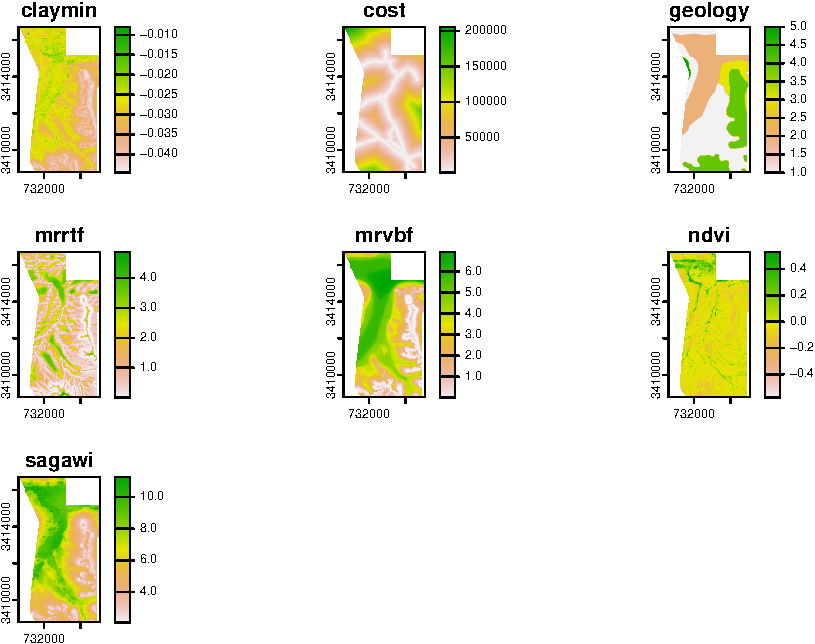
\includegraphics{Technical-Manual-Soil-Sampling-Design_files/figure-latex/fig-3-1.pdf}
\caption{\label{fig:fig-3}Covariates}
\end{figure}

\hypertarget{representativeness-of-the-legacy-soil-data}{%
\section{Representativeness of the Legacy Soil Data}\label{representativeness-of-the-legacy-soil-data}}

The next step involves the determination of the distributions of environmental values in the soil samples data and its comparison with the existing distributions of each environmental variable to determine the representativeness of the soil points in the environmental space.

The comparison of distributions is performed through the Kullback--Leibler divergence (KL) distance, a measure used to quantify the difference between two probability distributions.
KL--divergence compares an `objective' or reference probability distribution (here, the distribution of covariates in the complete covariate space -- P) with a `model' or approximate probability distribution (the space of covariates in the soil samples -- Q). The main idea is to determine how much information is lost when Q is used to approximate P. In other words, KL--divergence measures how much the Q distribution deviates from the P distribution. KL--divergence equals approaches to 0 as the two distributions have identical quantities of information.

We cross soil and environmental data to create a dataset with the values of the environmental parameters at the locations of the soil samples.

We first calculate a \texttt{\textquotesingle{}n–matrix\textquotesingle{}} with the values of the covariates dividing their distributions into \texttt{\textquotesingle{}n\textquotesingle{}} equally--spaced bins. Each bin captures the environmental variability within its interval in the total distribution. In this exercise, \texttt{\textquotesingle{}n\textquotesingle{}} equals to 25. The result is a 26×4 matrix, where the rows represent the upper and lower limit of the bin and (thus, 26 rows are required to represent 25 bins), and 4 correspond to the number of variables used as environmental proxies.

\begin{Shaded}
\begin{Highlighting}[]
  \DocumentationTok{\#\# Variability matrix in the covariates}
    \CommentTok{\# Define Number of bins}
\NormalTok{      nb }\OtherTok{\textless{}{-}} \DecValTok{25}
      \CommentTok{\#quantile matrix (of the covariate data)}
\NormalTok{      q.mat }\OtherTok{\textless{}{-}} \FunctionTok{matrix}\NormalTok{(}\ConstantTok{NA}\NormalTok{, }\AttributeTok{nrow=}\NormalTok{(nb}\SpecialCharTok{+}\DecValTok{1}\NormalTok{), }\AttributeTok{ncol=} \FunctionTok{nlyr}\NormalTok{(cov.dat))}
\NormalTok{      j}\OtherTok{=}\DecValTok{1}
      \ControlFlowTok{for}\NormalTok{ (i }\ControlFlowTok{in} \DecValTok{1}\SpecialCharTok{:}\FunctionTok{nlyr}\NormalTok{(cov.dat))\{ }\CommentTok{\#note the index start here}
      \CommentTok{\#get a quantile matrix together of the covariates}
\NormalTok{        ran1 }\OtherTok{\textless{}{-}} \FunctionTok{minmax}\NormalTok{(cov.dat[[i]])[}\DecValTok{2}\NormalTok{] }\SpecialCharTok{{-}} \FunctionTok{minmax}\NormalTok{(cov.dat[[i]])[}\DecValTok{1}\NormalTok{]}
\NormalTok{        step1 }\OtherTok{\textless{}{-}}\NormalTok{ ran1}\SpecialCharTok{/}\NormalTok{nb }
\NormalTok{        q.mat[,j] }\OtherTok{\textless{}{-}} \FunctionTok{seq}\NormalTok{(}\FunctionTok{minmax}\NormalTok{(cov.dat[[i]])[}\DecValTok{1}\NormalTok{], }\AttributeTok{to =} \FunctionTok{minmax}\NormalTok{(cov.dat[[i]])[}\DecValTok{2}\NormalTok{], }\AttributeTok{by =}\NormalTok{step1)}
\NormalTok{        j}\OtherTok{\textless{}{-}}\NormalTok{ j}\SpecialCharTok{+}\DecValTok{1}\NormalTok{\}}
\end{Highlighting}
\end{Shaded}

From this matrix, we compute the hypercube matrix of covariates in the whole covariate space.

\begin{Shaded}
\begin{Highlighting}[]
\DocumentationTok{\#\# Hypercube of "objective" distribution (P) – covariates}
  \CommentTok{\# Convert SpatRaster to dataframe for calculations}
\NormalTok{    cov.dat.df }\OtherTok{\textless{}{-}} \FunctionTok{as.data.frame}\NormalTok{(cov.dat) }
\NormalTok{    cov.mat }\OtherTok{\textless{}{-}} \FunctionTok{matrix}\NormalTok{(}\DecValTok{1}\NormalTok{, }\AttributeTok{nrow=}\NormalTok{nb, }\AttributeTok{ncol=}\FunctionTok{ncol}\NormalTok{(q.mat))}
      \ControlFlowTok{for}\NormalTok{ (i }\ControlFlowTok{in} \DecValTok{1}\SpecialCharTok{:}\FunctionTok{nrow}\NormalTok{(cov.dat.df))\{ }\CommentTok{\# the number of pixels}
\NormalTok{        cntj }\OtherTok{\textless{}{-}} \DecValTok{1} 
      \ControlFlowTok{for}\NormalTok{ (j }\ControlFlowTok{in} \DecValTok{1}\SpecialCharTok{:}\FunctionTok{ncol}\NormalTok{(cov.dat.df))\{ }\CommentTok{\#for each column}
\NormalTok{        dd}\OtherTok{\textless{}{-}}\NormalTok{ cov.dat.df[i,j]  }
        \ControlFlowTok{for}\NormalTok{ (k }\ControlFlowTok{in} \DecValTok{1}\SpecialCharTok{:}\NormalTok{nb)\{  }\CommentTok{\#for each quantile}
\NormalTok{          kl }\OtherTok{\textless{}{-}}\NormalTok{ q.mat[k, cntj] }
\NormalTok{          ku }\OtherTok{\textless{}{-}}\NormalTok{ q.mat[k}\SpecialCharTok{+}\DecValTok{1}\NormalTok{, cntj] }
          \ControlFlowTok{if}\NormalTok{ (}\FunctionTok{is.na}\NormalTok{(dd)) \{}
            \FunctionTok{print}\NormalTok{(}\StringTok{\textquotesingle{}Missing\textquotesingle{}}\NormalTok{)}
\NormalTok{          \}}
          \ControlFlowTok{else} \ControlFlowTok{if}\NormalTok{ (dd }\SpecialCharTok{\textgreater{}=}\NormalTok{ kl }\SpecialCharTok{\&}\NormalTok{ dd }\SpecialCharTok{\textless{}=}\NormalTok{ ku)\{cov.mat[k, cntj]}\OtherTok{\textless{}{-}}\NormalTok{ cov.mat[k, cntj] }\SpecialCharTok{+} \DecValTok{1}\NormalTok{\} }
\NormalTok{        \}}
\NormalTok{        cntj }\OtherTok{\textless{}{-}}\NormalTok{ cntj}\SpecialCharTok{+}\DecValTok{1}
\NormalTok{      \}}
\NormalTok{    \}}
\end{Highlighting}
\end{Shaded}

We then calculate the hypercube matrix of covariates in the sample space.

\begin{Shaded}
\begin{Highlighting}[]
\DocumentationTok{\#\# Sample data hypercube}
\NormalTok{  h.mat }\OtherTok{\textless{}{-}} \FunctionTok{matrix}\NormalTok{(}\DecValTok{1}\NormalTok{, }\AttributeTok{nrow=}\NormalTok{nb, }\AttributeTok{ncol=}\FunctionTok{ncol}\NormalTok{(q.mat))}
  
  \ControlFlowTok{for}\NormalTok{ (ii }\ControlFlowTok{in} \DecValTok{1}\SpecialCharTok{:}\FunctionTok{nrow}\NormalTok{(p.dat\_I))\{ }\CommentTok{\# the number of observations}
\NormalTok{    cntj }\OtherTok{\textless{}{-}} \DecValTok{1} 
    \ControlFlowTok{for}\NormalTok{ (jj }\ControlFlowTok{in} \DecValTok{2}\SpecialCharTok{:}\FunctionTok{ncol}\NormalTok{(p.dat\_I))\{ }\CommentTok{\#for each column}
\NormalTok{      dd }\OtherTok{\textless{}{-}}\NormalTok{ p.dat\_I[ii,jj]  }
      \ControlFlowTok{for}\NormalTok{ (kk }\ControlFlowTok{in} \DecValTok{1}\SpecialCharTok{:}\NormalTok{nb)\{  }\CommentTok{\#for each bin}
\NormalTok{        kl }\OtherTok{\textless{}{-}}\NormalTok{ q.mat[kk, cntj] }
\NormalTok{        ku }\OtherTok{\textless{}{-}}\NormalTok{ q.mat[kk}\SpecialCharTok{+}\DecValTok{1}\NormalTok{, cntj] }
        \ControlFlowTok{if}\NormalTok{ (dd }\SpecialCharTok{\textgreater{}=}\NormalTok{ kl }\SpecialCharTok{\&}\NormalTok{ dd }\SpecialCharTok{\textless{}=}\NormalTok{ ku)\{h.mat[kk, cntj] }\OtherTok{\textless{}{-}}\NormalTok{ h.mat[kk, cntj] }\SpecialCharTok{+} \DecValTok{1}\NormalTok{\}}
\NormalTok{      \}}
\NormalTok{      cntj }\OtherTok{\textless{}{-}}\NormalTok{ cntj}\SpecialCharTok{+}\DecValTok{1}
\NormalTok{    \}}
\NormalTok{  \}}
\end{Highlighting}
\end{Shaded}

\begin{itemize}
\tightlist
\item
  \textbf{KL--divergence}
\end{itemize}

We calculate the KL--divergence to measure how much the distribution of covariates in tbe sample space (Q) deviates from the distribution of covariates in the complete study area space (P).

\begin{Shaded}
\begin{Highlighting}[]
  \DocumentationTok{\#\# Compare covariate distributions in P and Q with Kullback–Leibler (KL) divergence}
\NormalTok{      kl.index }\OtherTok{\textless{}{-}}\FunctionTok{c}\NormalTok{()}
      \ControlFlowTok{for}\NormalTok{(i }\ControlFlowTok{in} \DecValTok{1}\SpecialCharTok{:}\FunctionTok{ncol}\NormalTok{(cov.dat.df))\{}
\NormalTok{        kl }\OtherTok{\textless{}{-}}    \FunctionTok{KL.empirical}\NormalTok{(}\FunctionTok{c}\NormalTok{(cov.mat[,i]), }\FunctionTok{c}\NormalTok{(h.mat[,i]))}
\NormalTok{        kl.index }\OtherTok{\textless{}{-}} \FunctionTok{c}\NormalTok{(kl.index,kl)}
\NormalTok{        klo }\OtherTok{\textless{}{-}}  \FunctionTok{mean}\NormalTok{(kl.index)}
\NormalTok{      \}}
      \CommentTok{\#print(kl.index) \# KL divergences of each covariate}
      \CommentTok{\#print(klo) \# KL divergence in the existing soil samples}
\end{Highlighting}
\end{Shaded}

The KL--divergence is always greater than or equal to zero, and reaches its minimum value (zero) only when P and Q are identical. Thus, lower values of KL--divergence are indicative of a good match between both the sample and the study area spaces, indicating that the sample space is a fair representation of the environmental conditions in the study area.

In this case, the KL--divergence value is 0.273, indicating that the legacy samples capture most of the environmental variability in the study area.

\begin{itemize}
\tightlist
\item
  \textbf{Percent of representativeness in relation to the overall environmental conditions}
\end{itemize}

Finally, we can also determine the degree in which our legacy soil dataset is representative of the existing environmental conditions in the study area. For that, we calculate the proportion of pixels in the study area that would fall within the convex hull polygon delineated upon the environmental conditions found at the soil legacy data locations only. The convex hull polygon is created upon a Principal Component transformation of the covariate data in the soil legacy data and using the outter limits of the scores of the points projected on the two main Components.

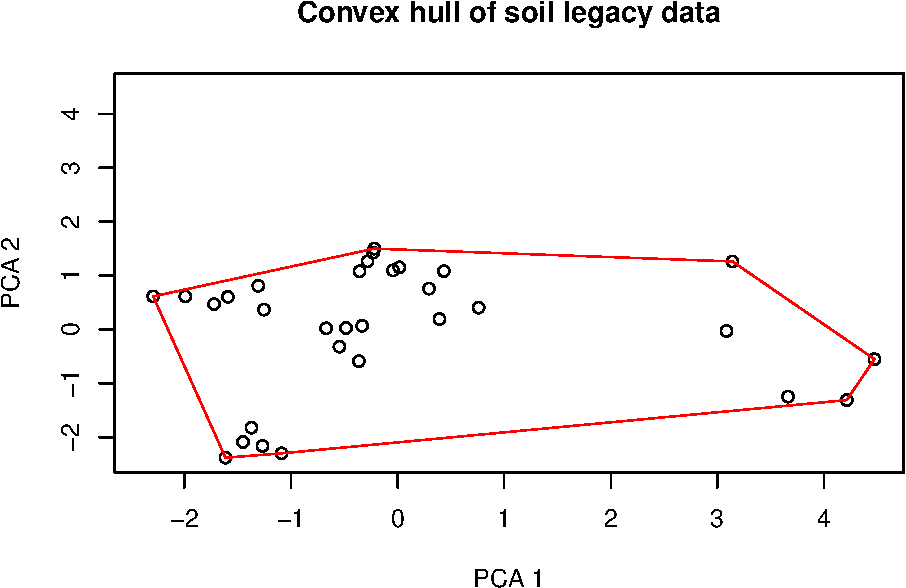
\includegraphics{Technical-Manual-Soil-Sampling-Design_files/figure-latex/fig-4-1.pdf} 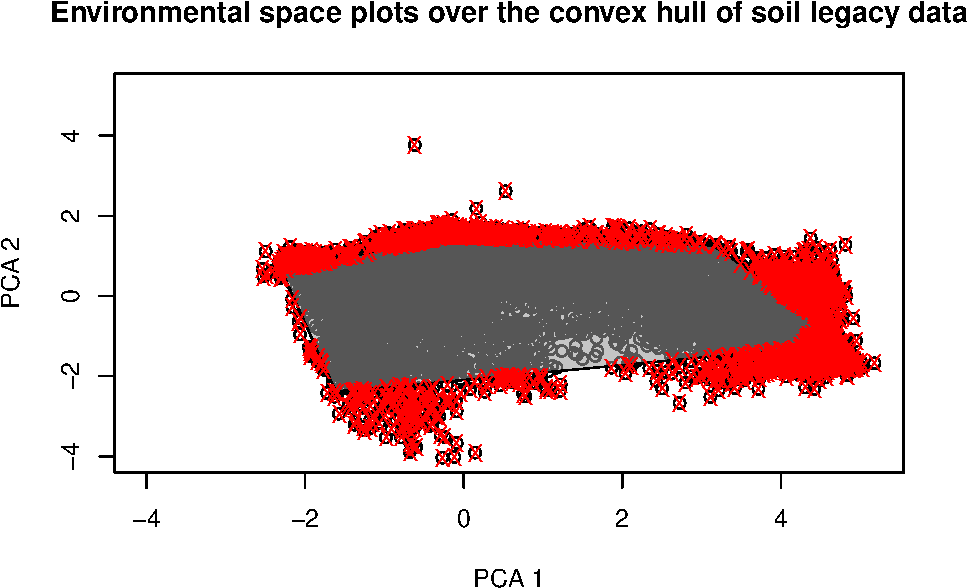
\includegraphics{Technical-Manual-Soil-Sampling-Design_files/figure-latex/fig-4-2.pdf}

This indicates that 83.8\% of the existing conditions in the study area fall within the convex hull delineated with the data in the soil samples, showing the level of adequacy of the proposed legacy data for DSM in the area.

\hypertarget{part-part-two-soil-sampling-design}{%
\part{Part two -- Soil Sampling Design}\label{part-part-two-soil-sampling-design}}

\hypertarget{determining-the-optimal-sampling-size}{%
\chapter{Determining the optimal sampling size}\label{determining-the-optimal-sampling-size}}

Several strategies exist for designing soil sampling, including regular, random, and stratified sampling. Each strategy comes with its own set of advantages and limitations, which must be carefully considered before commencing a soil sampling campaign. Regular sampling, also called grid sampling, is straightforward and ensures uniform coverage, making it suitable for spatial analysis and detecting trends. However, it may introduce bias and miss small--scale variability. Generally, random sampling may require a larger number of samples to accurately capture soil variability compared to stratified sampling, which is more targeted. Nonetheless, from a statistical standpoint, random sampling is often preferred. It effectively minimizes selection bias by giving every part of the study area an equal chance of being selected. This approach yields a sample that is truly representative of the entire population, leading to more accurate, broadly applicable conclusions. Random sampling also supports valid statistical inferences, ensures reliability of results, and simplifies the estimation of errors, thereby facilitating a broad spectrum of statistical analyses.

The determination of both the number and locations of soil samples is an important element in the success of any sampling campaign. The chosen strategy directly influences the representativeness and accuracy of the soil data collected, which in turn impacts the quality of the conclusions drawn from the study.

In this exercise, we make use of the data provided by (\protect\hyperlink{ref-Malone}{Malone, Minansy and Brungard, 2019}) with 4 raster covariates in a 100 has area. We want to determine the minimal number of soil samples that must be collated to capture at least the 95\% of variability within the environmental covariates. The procedure start with random distribution of a low number of samples in the area, determine the values of the spatial covariates, and compare them with those representing the whole diversity in the area at pixel scale. The comparisons are made using the \texttt{\textquotesingle{}Kullback–Leibler\ divergence\ (KL)\textquotesingle{}} -- a measure of how the probability distribution of the information in the samples is different from that of the Population, i.e.~the covariate space. We also calculate the \texttt{\textquotesingle{}\%\ of\ representativeness\textquotesingle{}} as the percent of variability in the covariate information for the complete area related to the variability of covariate information in the sample dataset. Further information can be found in the original work from (\protect\hyperlink{ref-Malone}{Malone, Minansy and Brungard, 2019}).

The initial section of the script is related to set--up options in the methodology. We load of R packages, define the working directory, load covariate data, and store it as \texttt{SpatRaster} object. Variables related to several aspects of the analyses, such as the aggregation factor of covariates (optional), the creation of a raster stack object(required in the \texttt{clhs} function), the initial and final number of samples in the trials, the increment step between trials, and the number of iterations within each trial, are also defined.

\begin{Shaded}
\begin{Highlighting}[]
  \DocumentationTok{\#\# Load raster covariate data}
    \CommentTok{\# Read Spatial data covariates as rasters with terra}
\NormalTok{    cov.dat }\OtherTok{\textless{}{-}}  \FunctionTok{list.files}\NormalTok{(raster.path, }\AttributeTok{pattern =} \StringTok{"tif$"}\NormalTok{,  }\AttributeTok{recursive =} \ConstantTok{TRUE}\NormalTok{, }\AttributeTok{full.names =} \ConstantTok{TRUE}\NormalTok{)}
\NormalTok{    cov.dat }\OtherTok{\textless{}{-}}\NormalTok{ terra}\SpecialCharTok{::}\FunctionTok{rast}\NormalTok{(cov.dat)}
    
    \CommentTok{\# Aggregate raster pixels to simplify data for calculations and build layer statistics}
\NormalTok{    cov.dat }\OtherTok{\textless{}{-}} \FunctionTok{aggregate}\NormalTok{(cov.dat, }\AttributeTok{fact=}\NormalTok{agg.factor, }\AttributeTok{fun=}\StringTok{"mean"}\NormalTok{)}
  
    \CommentTok{\# Create a raster stack}
\NormalTok{    cov.dat.ras }\OtherTok{\textless{}{-}}\NormalTok{ raster}\SpecialCharTok{::}\FunctionTok{stack}\NormalTok{(cov.dat) }
\end{Highlighting}
\end{Shaded}

We can see the covariates in a plot.

\begin{Shaded}
\begin{Highlighting}[]
   \FunctionTok{plot}\NormalTok{(cov.dat)}
\end{Highlighting}
\end{Shaded}

\begin{figure}
\centering
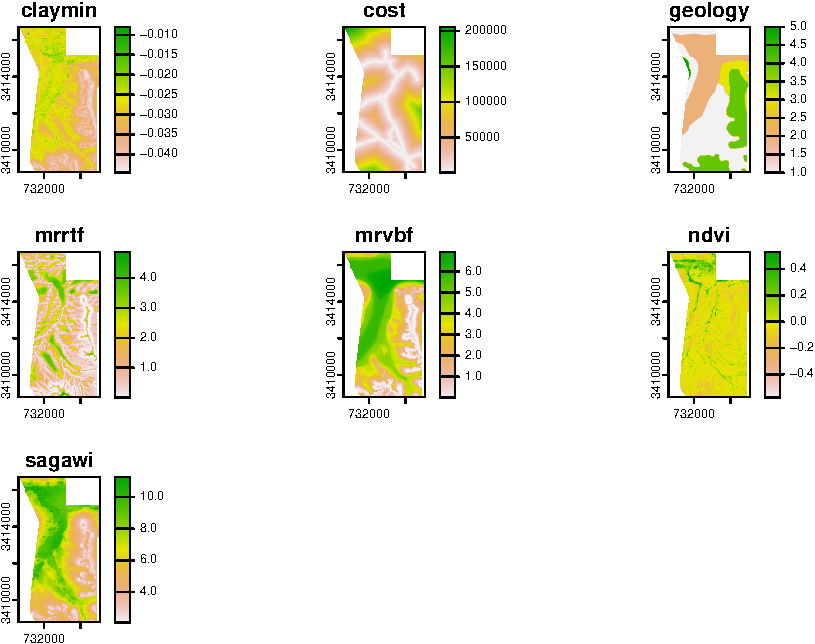
\includegraphics{Technical-Manual-Soil-Sampling-Design_files/figure-latex/fig-5-1.pdf}
\caption{\label{fig:fig-5}Plot of the covariates}
\end{figure}

\begin{Shaded}
\begin{Highlighting}[]
  \DocumentationTok{\#\# Define the number of samples to be tested in a loop (from initial to final) and the step of the sequence}
\NormalTok{  initial.n }\OtherTok{\textless{}{-}} \DecValTok{10}
\NormalTok{  final.n }\OtherTok{\textless{}{-}} \DecValTok{150}
\NormalTok{  by.n }\OtherTok{\textless{}{-}} \DecValTok{20}
\NormalTok{  iters }\OtherTok{\textless{}{-}} \DecValTok{2}
\end{Highlighting}
\end{Shaded}

The second section is where the analyses of divergence and representativeness of the sampling scheme are calculated.

The analyses are performed in a loop using growing numbers of samples at each trial. Some empty vectors are defined to store the output results at each loop. At each trial of sample size \texttt{\textquotesingle{}N\textquotesingle{}}, soil samples are located at locations where the amount of information in the covariates is maximized according to the conditioned Latin Hypercube sampling method in the \texttt{\textquotesingle{}clhs\textquotesingle{}} package (\protect\hyperlink{ref-Roudier2011}{Roudier \emph{et al.}, 2011}). A number of 2 replicates are calculated to determine the amount inter--variability in KL divergence and representativeness in the trial. The final results for each sample size correspond to the mean results obtained from each iteration at the corresponding sample size. The optimal sample size selected correspond to the minimum sample size that accounts for at least 95\% of the variability of information in the covariates within the area. The optimal sampling schema proposed correspond to the random scheme at the optimal sample size with higher value of representativeness.

\begin{Shaded}
\begin{Highlighting}[]
  \CommentTok{\# Define empty vectors to store results}
\NormalTok{  number\_of\_samples }\OtherTok{\textless{}{-}} \FunctionTok{c}\NormalTok{()}
\NormalTok{  prop\_explained }\OtherTok{\textless{}{-}} \FunctionTok{c}\NormalTok{()}
\NormalTok{  klo\_samples }\OtherTok{\textless{}{-}}\FunctionTok{c}\NormalTok{()}
\NormalTok{  samples\_storage }\OtherTok{\textless{}{-}} \FunctionTok{list}\NormalTok{()}

\ControlFlowTok{for}\NormalTok{ (trial }\ControlFlowTok{in} \FunctionTok{seq}\NormalTok{(initial.n, final.n, }\AttributeTok{by=}\NormalTok{by.n))\{}
 \ControlFlowTok{for}\NormalTok{ (iteration }\ControlFlowTok{in} \DecValTok{1}\SpecialCharTok{:}\NormalTok{iters)\{}
\NormalTok{    p.dat\_I }\OtherTok{\textless{}{-}} \FunctionTok{clhs}\NormalTok{(cov.dat.ras, }\AttributeTok{size =}\NormalTok{ trial, }\AttributeTok{iter =} \DecValTok{5000}\NormalTok{, }\AttributeTok{progress =} \ConstantTok{FALSE}\NormalTok{, }\AttributeTok{simple =} \ConstantTok{FALSE}\NormalTok{)}

    \CommentTok{\# Get covariate values for each point}
\NormalTok{    p.dat\_I }\OtherTok{\textless{}{-}}\NormalTok{ p.dat\_I}\SpecialCharTok{$}\NormalTok{sampled\_data}

  \CommentTok{\# Store samples in list}
\NormalTok{  samples\_storage[[}\FunctionTok{paste0}\NormalTok{(}\StringTok{"N"}\NormalTok{, trial,}\StringTok{"\_"}\NormalTok{,iteration)]] }\OtherTok{\textless{}{-}}\NormalTok{ p.dat\_I}

  \DocumentationTok{\#\# Comparison of population and sample distributions – Kullback–Leibler (KL) divergence}
    
    \CommentTok{\# Quantiles of the study area: Number of bins}
\NormalTok{    nb}\OtherTok{\textless{}{-}} \DecValTok{25}
    \CommentTok{\#quantile matrix (of the covariate data)}
\NormalTok{    q.mat}\OtherTok{\textless{}{-}} \FunctionTok{matrix}\NormalTok{(}\ConstantTok{NA}\NormalTok{, }\AttributeTok{nrow=}\NormalTok{(nb}\SpecialCharTok{+}\DecValTok{1}\NormalTok{), }\AttributeTok{ncol=} \FunctionTok{nlyr}\NormalTok{(cov.dat))}
\NormalTok{    j}\OtherTok{=}\DecValTok{1}
    \ControlFlowTok{for}\NormalTok{ (i }\ControlFlowTok{in} \DecValTok{1}\SpecialCharTok{:}\FunctionTok{nlyr}\NormalTok{(cov.dat))\{ }\CommentTok{\#note the index start here}
      \CommentTok{\#get a quantile matrix together of the covariates}
\NormalTok{      ran1 }\OtherTok{\textless{}{-}} \FunctionTok{minmax}\NormalTok{(cov.dat[[i]])[}\DecValTok{2}\NormalTok{] }\SpecialCharTok{{-}} \FunctionTok{minmax}\NormalTok{(cov.dat[[i]])[}\DecValTok{1}\NormalTok{]}
\NormalTok{      step1 }\OtherTok{\textless{}{-}}\NormalTok{ ran1}\SpecialCharTok{/}\NormalTok{nb }
\NormalTok{      q.mat[,j] }\OtherTok{\textless{}{-}} \FunctionTok{seq}\NormalTok{(}\FunctionTok{minmax}\NormalTok{(cov.dat[[i]])[}\DecValTok{1}\NormalTok{], }\AttributeTok{to =} \FunctionTok{minmax}\NormalTok{(cov.dat[[i]])[}\DecValTok{2}\NormalTok{], }\AttributeTok{by =}\NormalTok{step1)}
\NormalTok{      j }\OtherTok{\textless{}{-}}\NormalTok{ j}\SpecialCharTok{+}\DecValTok{1}\NormalTok{\}}
\NormalTok{    q.mat}
    
    \CommentTok{\# Hypercube of covariates in study area}
\NormalTok{    cov.dat.df }\OtherTok{\textless{}{-}} \FunctionTok{as.data.frame}\NormalTok{(cov.dat) }\CommentTok{\# convert SpatRaster to dataframe}
\NormalTok{    cov.mat }\OtherTok{\textless{}{-}} \FunctionTok{matrix}\NormalTok{(}\DecValTok{1}\NormalTok{, }\AttributeTok{nrow=}\NormalTok{nb, }\AttributeTok{ncol=}\FunctionTok{ncol}\NormalTok{(q.mat))}
    \ControlFlowTok{for}\NormalTok{ (i }\ControlFlowTok{in} \DecValTok{1}\SpecialCharTok{:}\FunctionTok{nrow}\NormalTok{(cov.dat.df))\{ }\CommentTok{\# the number of pixels}
\NormalTok{      cntj }\OtherTok{\textless{}{-}} \DecValTok{1} 
      \ControlFlowTok{for}\NormalTok{ (j }\ControlFlowTok{in} \DecValTok{1}\SpecialCharTok{:}\FunctionTok{ncol}\NormalTok{(cov.dat.df))\{ }\CommentTok{\#for each column}
\NormalTok{        dd }\OtherTok{\textless{}{-}}\NormalTok{ cov.dat.df[i,j]  }
        \ControlFlowTok{for}\NormalTok{ (k }\ControlFlowTok{in} \DecValTok{1}\SpecialCharTok{:}\NormalTok{nb)\{  }\CommentTok{\#for each quantile}
\NormalTok{          kl }\OtherTok{\textless{}{-}}\NormalTok{ q.mat[k, cntj] }
\NormalTok{          ku }\OtherTok{\textless{}{-}}\NormalTok{ q.mat[k}\SpecialCharTok{+}\DecValTok{1}\NormalTok{, cntj] }
          \ControlFlowTok{if}\NormalTok{ (}\FunctionTok{is.na}\NormalTok{(dd)) \{}
            \FunctionTok{print}\NormalTok{(}\FunctionTok{paste}\NormalTok{(}\StringTok{\textquotesingle{}N\_\textquotesingle{}}\NormalTok{,trial,}\StringTok{\textquotesingle{}\_\textquotesingle{}}\NormalTok{,iteration,}\StringTok{\textquotesingle{}Missing\textquotesingle{}}\NormalTok{))}
\NormalTok{          \}}
          \ControlFlowTok{else} \ControlFlowTok{if}\NormalTok{ (dd }\SpecialCharTok{\textgreater{}=}\NormalTok{ kl }\SpecialCharTok{\&}\NormalTok{ dd }\SpecialCharTok{\textless{}=}\NormalTok{ ku)\{cov.mat[k, cntj]}\OtherTok{\textless{}{-}}\NormalTok{ cov.mat[k, cntj] }\SpecialCharTok{+} \DecValTok{1}\NormalTok{\} }
\NormalTok{        \}}
\NormalTok{        cntj }\OtherTok{\textless{}{-}}\NormalTok{ cntj}\SpecialCharTok{+}\DecValTok{1}
\NormalTok{      \}}
\NormalTok{    \}}
\NormalTok{    cov.mat}

    \CommentTok{\# Compare whole study area covariate space with the selected sample}
    \CommentTok{\# Sample data hypercube (essentially the same script as for the grid data but just doing it on the sample data)}
\NormalTok{    h.mat }\OtherTok{\textless{}{-}} \FunctionTok{matrix}\NormalTok{(}\DecValTok{1}\NormalTok{, }\AttributeTok{nrow=}\NormalTok{nb, }\AttributeTok{ncol=}\FunctionTok{ncol}\NormalTok{(q.mat))}
    
    \ControlFlowTok{for}\NormalTok{ (ii }\ControlFlowTok{in} \DecValTok{1}\SpecialCharTok{:}\FunctionTok{nrow}\NormalTok{(p.dat\_I))\{ }\CommentTok{\# the number of observations}
\NormalTok{      cntj }\OtherTok{\textless{}{-}} \DecValTok{1} 
      \ControlFlowTok{for}\NormalTok{ (jj }\ControlFlowTok{in} \DecValTok{1}\SpecialCharTok{:}\FunctionTok{ncol}\NormalTok{(p.dat\_I))\{ }\CommentTok{\#for each column}
\NormalTok{        dd }\OtherTok{\textless{}{-}} \FunctionTok{as.data.frame}\NormalTok{(p.dat\_I)[ii,jj]  }
        \ControlFlowTok{for}\NormalTok{ (kk }\ControlFlowTok{in} \DecValTok{1}\SpecialCharTok{:}\NormalTok{nb)\{  }\CommentTok{\#for each quantile}
\NormalTok{          kl }\OtherTok{\textless{}{-}}\NormalTok{ q.mat[kk, cntj] }
\NormalTok{          ku }\OtherTok{\textless{}{-}}\NormalTok{ q.mat[kk}\SpecialCharTok{+}\DecValTok{1}\NormalTok{, cntj] }
          \ControlFlowTok{if}\NormalTok{ (dd }\SpecialCharTok{\textgreater{}=}\NormalTok{ kl }\SpecialCharTok{\&}\NormalTok{ dd }\SpecialCharTok{\textless{}=}\NormalTok{ ku)\{h.mat[kk, cntj]}\OtherTok{\textless{}{-}}\NormalTok{ h.mat[kk, cntj] }\SpecialCharTok{+} \DecValTok{1}\NormalTok{\}}
\NormalTok{        \}}
\NormalTok{        cntj }\OtherTok{\textless{}{-}}\NormalTok{ cntj}\SpecialCharTok{+}\DecValTok{1}
\NormalTok{      \}}
\NormalTok{    \}}
\NormalTok{    h.mat }
    
    
    \DocumentationTok{\#\# Compute Kullback{-}Leibler (KL) divergence}
\NormalTok{    kl.index }\OtherTok{\textless{}{-}} \FunctionTok{c}\NormalTok{()}
    \ControlFlowTok{for}\NormalTok{(i }\ControlFlowTok{in} \DecValTok{1}\SpecialCharTok{:}\FunctionTok{ncol}\NormalTok{(cov.dat.df))\{}
\NormalTok{      kl }\OtherTok{\textless{}{-}} \FunctionTok{KL.empirical}\NormalTok{(}\FunctionTok{c}\NormalTok{(cov.mat[,i]), }\FunctionTok{c}\NormalTok{(h.mat[,i]))}
\NormalTok{      kl.index }\OtherTok{\textless{}{-}} \FunctionTok{c}\NormalTok{(kl.index,kl)}
\NormalTok{      klo }\OtherTok{\textless{}{-}}  \FunctionTok{mean}\NormalTok{(kl.index)}
\NormalTok{    \}}
  
    \DocumentationTok{\#\# Similarity of the Legacy Dataset: {-}{-}{-}{-}}
    \DocumentationTok{\#\# Calculate the proportion of "env. variables" in the covariate spectra that fall within the convex hull of variables in the "environmental sample space"}
    \CommentTok{\# Principal component of the legacy data sample}
\NormalTok{    pca.s }\OtherTok{=} \FunctionTok{prcomp}\NormalTok{(}\FunctionTok{data.frame}\NormalTok{(p.dat\_I}\SpecialCharTok{@}\NormalTok{data),}\AttributeTok{scale=}\ConstantTok{TRUE}\NormalTok{, }\AttributeTok{center=}\ConstantTok{TRUE}\NormalTok{)}
\NormalTok{    scores\_pca1 }\OtherTok{=} \FunctionTok{as.data.frame}\NormalTok{(pca.s}\SpecialCharTok{$}\NormalTok{x)}
    \CommentTok{\# Plot the first 2 principal components and convex hull}
\NormalTok{    rand.tr }\OtherTok{\textless{}{-}} \FunctionTok{tri.mesh}\NormalTok{(scores\_pca1[,}\DecValTok{1}\NormalTok{],scores\_pca1[,}\DecValTok{2}\NormalTok{],}\StringTok{"remove"}\NormalTok{) }\CommentTok{\# Delaunay triangulation }
\NormalTok{    rand.ch }\OtherTok{\textless{}{-}} \FunctionTok{convex.hull}\NormalTok{(rand.tr, }\AttributeTok{plot.it=}\NormalTok{F) }\CommentTok{\# convex hull}
\NormalTok{    pr\_poly }\OtherTok{\textless{}{-}} \FunctionTok{cbind}\NormalTok{(}\AttributeTok{x=}\FunctionTok{c}\NormalTok{(rand.ch}\SpecialCharTok{$}\NormalTok{x),}\AttributeTok{y=}\FunctionTok{c}\NormalTok{(rand.ch}\SpecialCharTok{$}\NormalTok{y)) }\CommentTok{\# save the convex hull vertices}
    \CommentTok{\# plot(scores\_pca1[,1], scores\_pca1[,2], xlab="PCA 1", ylab="PCA 2", xlim=c(min(scores\_pca1[,1:2]), max(scores\_pca1[,1:2])),ylim=c(min(scores\_pca1[,1:2]), max(scores\_pca1[,1:2])), main=\textquotesingle{}Convex hull of soil legacy data\textquotesingle{})}
    \CommentTok{\# lines(c(rand.ch$x,rand.ch$x[1]), c(rand.ch$y,rand.ch$y[1]),col="red",lwd=1) \# draw the convex hull (domain of legacy data)}
    
    \CommentTok{\# PCA projection of study area population onto the principal components}
\NormalTok{    PCA\_projection }\OtherTok{\textless{}{-}} \FunctionTok{predict}\NormalTok{(pca.s, cov.dat.df) }\CommentTok{\# Project study area population onto sample PC}
\NormalTok{    newScores }\OtherTok{=} \FunctionTok{cbind}\NormalTok{(}\AttributeTok{x=}\NormalTok{PCA\_projection[,}\DecValTok{1}\NormalTok{],}\AttributeTok{y=}\NormalTok{PCA\_projection[,}\DecValTok{2}\NormalTok{]) }\CommentTok{\# PC scores of projected population}
    \CommentTok{\# Check which points fall within the polygon}
\NormalTok{    pip }\OtherTok{\textless{}{-}} \FunctionTok{point.in.polygon}\NormalTok{(newScores[,}\DecValTok{2}\NormalTok{], newScores[,}\DecValTok{1}\NormalTok{], pr\_poly[,}\DecValTok{2}\NormalTok{],pr\_poly[,}\DecValTok{1}\NormalTok{],}\AttributeTok{mode.checked=}\ConstantTok{FALSE}\NormalTok{)}
\NormalTok{    newScores }\OtherTok{\textless{}{-}} \FunctionTok{data.frame}\NormalTok{(}\FunctionTok{cbind}\NormalTok{(newScores, pip))}
    \CommentTok{\# Plot the polygon and all points to be checked}
    \CommentTok{\# if(trial == final.n)\{}
    \CommentTok{\# plot(newScores, xlab="PCA 1", ylab="PCA 2", xlim=c(min(newScores[,1:2]), max(newScores[,1:2])), ylim=c(min(newScores[,1:2]), max(newScores[,1:2])), col=\textquotesingle{}black\textquotesingle{}, main=\textquotesingle{}Environmental space plots over the convex hull of soil legacy data\textquotesingle{})}
    \CommentTok{\# polygon(pr\_poly,col=\textquotesingle{}\#99999990\textquotesingle{})}
    \CommentTok{\# \# Plot points outside convex hull  }
    \CommentTok{\# points(newScores[which(newScores$pip==0),1:2],pch=\textquotesingle{}X\textquotesingle{}, col=\textquotesingle{}red\textquotesingle{})}
    \CommentTok{\# \}}
    \CommentTok{\# Proportion of the conditions in the study area that fall within the convex hull}
    \CommentTok{\#sum(newScores$pip)/nrow(newScores)*100 }
\NormalTok{  klo\_samples }\OtherTok{\textless{}{-}} \FunctionTok{c}\NormalTok{(klo\_samples,klo)}
\NormalTok{  prop\_explained }\OtherTok{\textless{}{-}} \FunctionTok{c}\NormalTok{(prop\_explained,}\FunctionTok{sum}\NormalTok{(newScores}\SpecialCharTok{$}\NormalTok{pip)}\SpecialCharTok{/}\FunctionTok{nrow}\NormalTok{(newScores)}\SpecialCharTok{*}\DecValTok{100}\NormalTok{)}
\NormalTok{number\_of\_samples }\OtherTok{\textless{}{-}} \FunctionTok{c}\NormalTok{(number\_of\_samples,trial)}
\CommentTok{\#print(paste("N samples = ",trial, " out of ",final.n, "; iteration = ",iteration,"; KL = ", klo, "; Proportion = ", sum(newScores$pip)/nrow(newScores)*100 ))}
\NormalTok{  \}}
\NormalTok{\}}
\end{Highlighting}
\end{Shaded}

Figure \ref{fig:fig-7} shows the distribution of covariates in the sample space, and Figure \ref{fig:fig-7a} indicates the variability in the estimations of KL divergence and repressentativeness percent in the 2 within each sample size.

\begin{Shaded}
\begin{Highlighting}[]
  \CommentTok{\# Plot the polygon and all points to be checked}
     \FunctionTok{plot}\NormalTok{(newScores[,}\DecValTok{1}\SpecialCharTok{:}\DecValTok{2}\NormalTok{], }\AttributeTok{xlab=}\StringTok{"PCA 1"}\NormalTok{, }\AttributeTok{ylab=}\StringTok{"PCA 2"}\NormalTok{, }\AttributeTok{xlim=}\FunctionTok{c}\NormalTok{(}\FunctionTok{min}\NormalTok{(newScores[,}\DecValTok{1}\SpecialCharTok{:}\DecValTok{2}\NormalTok{]), }\FunctionTok{max}\NormalTok{(newScores[,}\DecValTok{1}\SpecialCharTok{:}\DecValTok{2}\NormalTok{])), }\AttributeTok{ylim=}\FunctionTok{c}\NormalTok{(}\FunctionTok{min}\NormalTok{(newScores[,}\DecValTok{1}\SpecialCharTok{:}\DecValTok{2}\NormalTok{]), }\FunctionTok{max}\NormalTok{(newScores[,}\DecValTok{1}\SpecialCharTok{:}\DecValTok{2}\NormalTok{])),}
          \AttributeTok{col=}\StringTok{\textquotesingle{}black\textquotesingle{}}\NormalTok{, }\AttributeTok{main=}\StringTok{\textquotesingle{}Environmental space plots over the convex hull of soil legacy data\textquotesingle{}}\NormalTok{)}
     \FunctionTok{polygon}\NormalTok{(pr\_poly,}\AttributeTok{col=}\StringTok{\textquotesingle{}\#99999990\textquotesingle{}}\NormalTok{)}
  \CommentTok{\# \# Plot points outside convex hull  }
     \FunctionTok{points}\NormalTok{(newScores[}\FunctionTok{which}\NormalTok{(newScores}\SpecialCharTok{$}\NormalTok{pip}\SpecialCharTok{==}\DecValTok{0}\NormalTok{),}\DecValTok{1}\SpecialCharTok{:}\DecValTok{2}\NormalTok{], }\AttributeTok{col=}\StringTok{\textquotesingle{}red\textquotesingle{}}\NormalTok{, }\AttributeTok{pch=}\DecValTok{12}\NormalTok{, }\AttributeTok{cex =}\DecValTok{1}\NormalTok{)}
\end{Highlighting}
\end{Shaded}

\begin{figure}
\centering
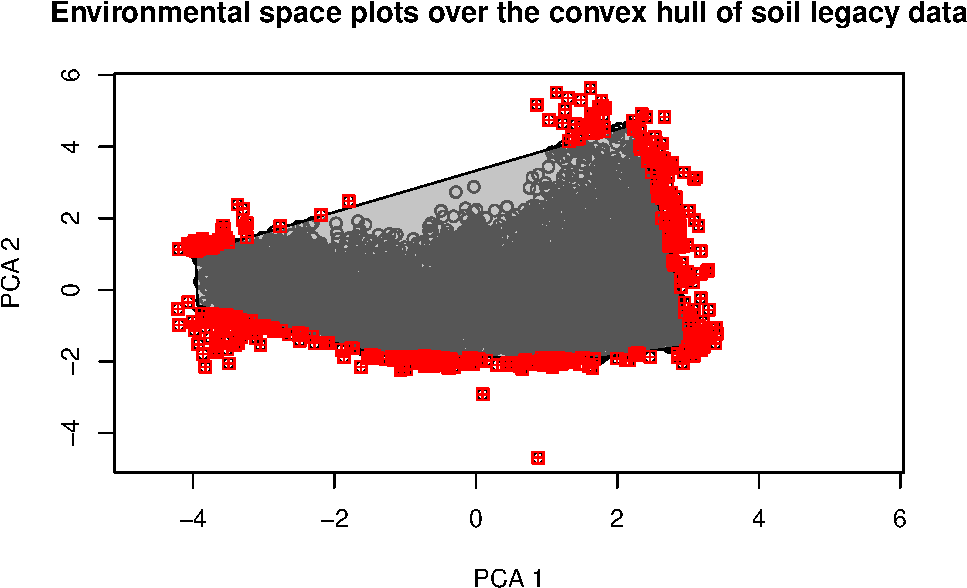
\includegraphics{Technical-Manual-Soil-Sampling-Design_files/figure-latex/fig-7-1.pdf}
\caption{\label{fig:fig-7}Distribution of covariates in the sample space}
\end{figure}

\begin{Shaded}
\begin{Highlighting}[]
  \DocumentationTok{\#\# Plot dispersion on KL and \% by N}
  \FunctionTok{par}\NormalTok{(}\AttributeTok{mar=}\FunctionTok{c}\NormalTok{(}\DecValTok{5}\NormalTok{, }\DecValTok{4}\NormalTok{, }\DecValTok{1}\NormalTok{, }\DecValTok{6}\NormalTok{))}
  \FunctionTok{boxplot}\NormalTok{(Perc }\SpecialCharTok{\textasciitilde{}}\NormalTok{ N, }\AttributeTok{data=}\NormalTok{results, }\AttributeTok{col =} \FunctionTok{rgb}\NormalTok{(}\DecValTok{1}\NormalTok{, }\FloatTok{0.1}\NormalTok{, }\DecValTok{0}\NormalTok{, }\AttributeTok{alpha =} \FloatTok{0.5}\NormalTok{),}\AttributeTok{ylab =} \StringTok{"\%"}\NormalTok{)}
  \FunctionTok{mtext}\NormalTok{(}\StringTok{"KL divergence"}\NormalTok{,}\AttributeTok{side=}\DecValTok{4}\NormalTok{,}\AttributeTok{line=}\DecValTok{3}\NormalTok{)}
  \CommentTok{\# Add new plot}
  \FunctionTok{par}\NormalTok{(}\AttributeTok{new =} \ConstantTok{TRUE}\NormalTok{,}\AttributeTok{mar=}\FunctionTok{c}\NormalTok{(}\DecValTok{5}\NormalTok{, }\DecValTok{4}\NormalTok{, }\DecValTok{1}\NormalTok{, }\DecValTok{6}\NormalTok{))}
  \CommentTok{\# Box plot}
  \FunctionTok{boxplot}\NormalTok{(KL }\SpecialCharTok{\textasciitilde{}}\NormalTok{ N, }\AttributeTok{data=}\NormalTok{results, }\AttributeTok{axes =} \ConstantTok{FALSE}\NormalTok{,}\AttributeTok{outline =} \ConstantTok{FALSE}\NormalTok{,}
          \AttributeTok{col =} \FunctionTok{rgb}\NormalTok{(}\DecValTok{0}\NormalTok{, }\FloatTok{0.8}\NormalTok{, }\DecValTok{1}\NormalTok{, }\AttributeTok{alpha =} \FloatTok{0.5}\NormalTok{), }\AttributeTok{ylab =} \StringTok{""}\NormalTok{)}
  \FunctionTok{axis}\NormalTok{(}\DecValTok{4}\NormalTok{, }\AttributeTok{at=}\FunctionTok{seq}\NormalTok{(}\FloatTok{0.02}\NormalTok{, }\FloatTok{0.36}\NormalTok{, }\AttributeTok{by=}\NormalTok{.}\DecValTok{06}\NormalTok{),  }\AttributeTok{label=}\FunctionTok{seq}\NormalTok{(}\FloatTok{0.02}\NormalTok{, }\FloatTok{0.36}\NormalTok{, }\AttributeTok{by=}\NormalTok{.}\DecValTok{06}\NormalTok{), }\AttributeTok{las=}\DecValTok{3}\NormalTok{)}
\end{Highlighting}
\end{Shaded}

\begin{figure}
\centering
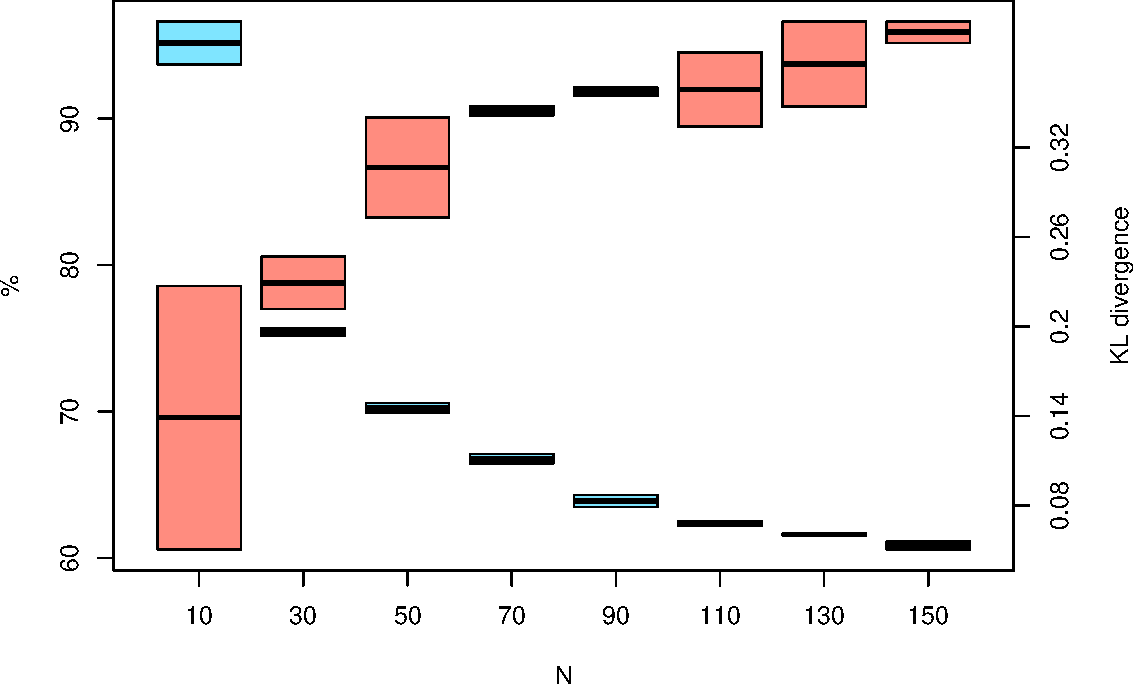
\includegraphics{Technical-Manual-Soil-Sampling-Design_files/figure-latex/fig-7a-1.pdf}
\caption{\label{fig:fig-7a}Boxplot of the dispersion in KLO and \% repressentativeness in the iteration trials for each sample size}
\end{figure}

We determine the optimal sample size and plot the evaluation results.

The following figure shows the cumulative distribution function (cdf) of the KL divergence and the \% of representativeness with growing sample sizes. Representativeness increases with the increasing sample size, while KL divergence decreases as expected. The red dot identifies the trial with the optimal sample size for the area in relation to the covariates analysed.

\begin{Shaded}
\begin{Highlighting}[]
  \DocumentationTok{\#\# Plot cdf and optimal sampling point}
\NormalTok{  x }\OtherTok{\textless{}{-}}\NormalTok{ xx}
\NormalTok{  y }\OtherTok{\textless{}{-}}\NormalTok{ normalized}
  
\NormalTok{  mydata }\OtherTok{\textless{}{-}} \FunctionTok{data.frame}\NormalTok{(x,y)}
\NormalTok{  opti }\OtherTok{\textless{}{-}}\NormalTok{ mydata[mydata}\SpecialCharTok{$}\NormalTok{x}\SpecialCharTok{==}\NormalTok{minimum\_n,]}
  
  \FunctionTok{plot\_ly}\NormalTok{(mydata,}
          \AttributeTok{x =} \SpecialCharTok{\textasciitilde{}}\NormalTok{x,}
          \AttributeTok{y =} \SpecialCharTok{\textasciitilde{}}\NormalTok{normalized,}
          \AttributeTok{mode =} \StringTok{"lines+markers"}\NormalTok{,}
          \AttributeTok{type =} \StringTok{"scatter"}\NormalTok{,}
          \AttributeTok{name =} \StringTok{"CDF (1–KL divergence)"}\NormalTok{) }\SpecialCharTok{\%\textgreater{}\%}
    \FunctionTok{add\_trace}\NormalTok{(}\AttributeTok{x =} \SpecialCharTok{\textasciitilde{}}\NormalTok{x,}
              \AttributeTok{y =} \SpecialCharTok{\textasciitilde{}}\NormalTok{jj,}
              \AttributeTok{mode =} \StringTok{"lines+markers"}\NormalTok{,}
              \AttributeTok{type =} \StringTok{"scatter"}\NormalTok{,}
              \AttributeTok{yaxis =} \StringTok{"y2"}\NormalTok{,}
              \AttributeTok{name =} \StringTok{"KL divergence"}\NormalTok{)  }\SpecialCharTok{\%\textgreater{}\%}
    \FunctionTok{add\_trace}\NormalTok{(}\AttributeTok{x =} \SpecialCharTok{\textasciitilde{}}\NormalTok{opti}\SpecialCharTok{$}\NormalTok{x,}
              \AttributeTok{y =} \SpecialCharTok{\textasciitilde{}}\NormalTok{opti}\SpecialCharTok{$}\NormalTok{y,}
              \AttributeTok{yaxis =} \StringTok{"y"}\NormalTok{,}
              \AttributeTok{mode =} \StringTok{"markers"}\NormalTok{,}
              \AttributeTok{name =} \StringTok{"Optimal N"}\NormalTok{,}
              \AttributeTok{marker =} \FunctionTok{list}\NormalTok{(}\AttributeTok{size =} \DecValTok{8}\NormalTok{, }\AttributeTok{color =} \StringTok{\textquotesingle{}\#d62728\textquotesingle{}}\NormalTok{,}\AttributeTok{line =} \FunctionTok{list}\NormalTok{(}\AttributeTok{color =} \StringTok{\textquotesingle{}black\textquotesingle{}}\NormalTok{, }\AttributeTok{width =} \DecValTok{1}\NormalTok{))) }\SpecialCharTok{\%\textgreater{}\%}
    \FunctionTok{layout}\NormalTok{(}\AttributeTok{xaxis =} \FunctionTok{list}\NormalTok{(}\AttributeTok{title =} \StringTok{"N"}\NormalTok{, }
                        \AttributeTok{showgrid =}\NormalTok{ T, }
                        \AttributeTok{dtick =} \DecValTok{50}\NormalTok{, }
                        \AttributeTok{tickfont =} \FunctionTok{list}\NormalTok{(}\AttributeTok{size =} \DecValTok{11}\NormalTok{)),}
           \AttributeTok{yaxis =} \FunctionTok{list}\NormalTok{(}\AttributeTok{title =} \StringTok{"KL divergence"}\NormalTok{, }\AttributeTok{showgrid =}\NormalTok{ F ),}
           \AttributeTok{yaxis2 =} \FunctionTok{list}\NormalTok{(}\AttributeTok{title =} \StringTok{"1–KL divergence (\% CDF)"}\NormalTok{,}
                         \AttributeTok{overlaying =} \StringTok{"y"}\NormalTok{, }\AttributeTok{side =} \StringTok{"right"}\NormalTok{),}
           \AttributeTok{legend =} \FunctionTok{list}\NormalTok{(}\AttributeTok{orientation =} \StringTok{"h"}\NormalTok{, }\AttributeTok{y =} \FloatTok{1.2}\NormalTok{, }\AttributeTok{x =} \FloatTok{0.1}\NormalTok{,}
                         \AttributeTok{traceorder =} \StringTok{"normal"}\NormalTok{),}
           \AttributeTok{margin =} \FunctionTok{list}\NormalTok{(}\AttributeTok{t =} \DecValTok{50}\NormalTok{, }\AttributeTok{b =} \DecValTok{50}\NormalTok{, }\AttributeTok{r =} \DecValTok{100}\NormalTok{, }\AttributeTok{l =} \DecValTok{80}\NormalTok{),}
           \AttributeTok{hovermode =} \StringTok{\textquotesingle{}x\textquotesingle{}}\NormalTok{)  }\SpecialCharTok{\%\textgreater{}\%} 
    \FunctionTok{config}\NormalTok{(}\AttributeTok{displayModeBar =} \ConstantTok{FALSE}\NormalTok{) }
\end{Highlighting}
\end{Shaded}

\begin{verbatim}
## PhantomJS not found. You can install it with webshot::install_phantomjs(). If it is installed, please make sure the phantomjs executable can be found via the PATH variable.
\end{verbatim}

\label{fig:fig-8}KL Divergence and Proportion of Representativeness as function of sample size

According to Figure \ref{fig:fig-8}, the minimum sampling size for the area, which captures at least 95\% of the environmental variability of covariates is N = 81.

Finally, we can determine the optimal distribution of samples over the study area according to these specific results, taking into account the minimum sampling size and the increasing interval in the sample size. The results are shown in Figure \ref{fig:fig-9}.

\begin{Shaded}
\begin{Highlighting}[]
\DocumentationTok{\#\# Determine the optimal iteration according to the optimal N size }
\NormalTok{  optimal\_iteration }\OtherTok{\textless{}{-}}\NormalTok{ results[}\FunctionTok{which}\NormalTok{(}\FunctionTok{abs}\NormalTok{(results}\SpecialCharTok{$}\NormalTok{N }\SpecialCharTok{{-}}\NormalTok{ minimum\_n) }\SpecialCharTok{==} \FunctionTok{min}\NormalTok{(}\FunctionTok{abs}\NormalTok{(results}\SpecialCharTok{$}\NormalTok{N }\SpecialCharTok{{-}}\NormalTok{ minimum\_n))),] }\SpecialCharTok{\%\textgreater{}\%}
    \FunctionTok{mutate}\NormalTok{(}\AttributeTok{IDX =} \DecValTok{1}\SpecialCharTok{:}\FunctionTok{n}\NormalTok{()) }\SpecialCharTok{\%\textgreater{}\%}
    \FunctionTok{filter}\NormalTok{(Perc}\SpecialCharTok{==}\FunctionTok{max}\NormalTok{(Perc)) }
  
  \CommentTok{\# Plot best iteration points}
\NormalTok{  N\_final }\OtherTok{\textless{}{-}}\NormalTok{ samples\_storage[}\FunctionTok{paste0}\NormalTok{(}\StringTok{"N"}\NormalTok{,optimal\_iteration}\SpecialCharTok{$}\NormalTok{N,}\StringTok{"\_"}\NormalTok{, optimal\_iteration}\SpecialCharTok{$}\NormalTok{IDX)][[}\DecValTok{1}\NormalTok{]]}
  \FunctionTok{plot}\NormalTok{(cov.dat[[}\DecValTok{1}\NormalTok{]])}
  \FunctionTok{points}\NormalTok{(N\_final)}
\end{Highlighting}
\end{Shaded}

\begin{figure}
\centering
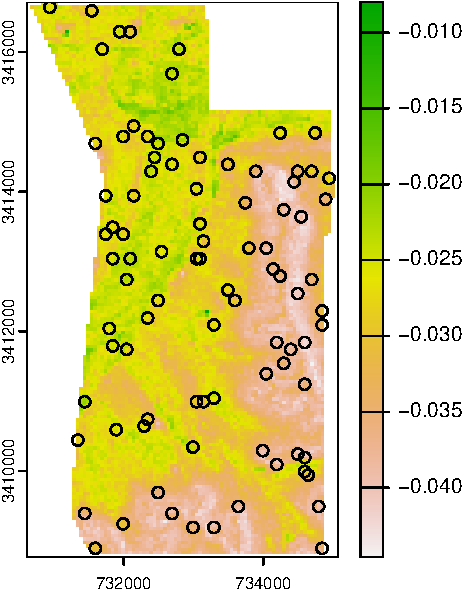
\includegraphics{Technical-Manual-Soil-Sampling-Design_files/figure-latex/fig-9-1.pdf}
\caption{\label{fig:fig-9}Covariates and optimal number and distribution of samples}
\end{figure}

In summary, we utilize the variability within the covariate data to ascertain the minimum number of samples required to capture a minimum of 95\% of this variability. Our approach involves assessing the similarities in variability between the sample space and the population space (study area) through calculations of the Kullback--Leibler (KL) divergence and the percentage of similarity at various stages of increasing sample sizes. These results are then utilized to fit a model representing the expected distribution of representativeness as a function of sample size. This model guides us in determining the minimum sample size necessary to achieve a representation of at least 95\% of the environmental diversity within the area

\hypertarget{stratified-sampling-design}{%
\chapter{Stratified Sampling Design}\label{stratified-sampling-design}}

Stratified random sampling is a technique where the study area is divided into different \texttt{groups} or \texttt{strata} based on certain environmental traits and a number of random samples are taken from within each group. One of the primary advantages of stratified sampling is its ability to capture the diversity within a population by making sure each group is represented. It can provide a more accurate reflection of the entire population compared to random sampling, especially when the groups are distinct and have unique qualities. This approach is particularly beneficial when certain subgroups within the population are specifically noteworthy. It also allows for more precise estimates with a smaller total sample size compared to simple random choice. Stratified sampling presents some disadvantages. Achieving effective categories requires a proper definition and delineation of the initial information to create the \texttt{strata}. The classification of the environmental information into categories and ensuring fair portrayal of each can be intricate and time--taking and mislabeling elements into an improper group can lead to skewed outcomes.

\hypertarget{general-procedure}{%
\section{General Procedure}\label{general-procedure}}

The creation of a stratified random sampling design involves the identification of relevant features describing the environmental diversity in the area (soil and land use are the environmental variables generally used to define strata), delineation of the strata, determination of the number of samples to distribute to each stratum, followed by random sampling within it. By identifying relevant classes, combining them to define strata and allocating an appropriate number of samples to each stratum, a representative sample can be obtained. Random sampling within each stratum helps to ensure that the sample is unbiased and provides a fair representation of the overall conditions in the area.

The first question is about how many samples must be retrieved from each strata. The sampling scheme starts with the definition of the total number of samples to collect. In this case, the determination of the sample size is a complex and highly variable process based, among others, on the specific goals of the study, the variability of environmental proxies, the statistical requirements for accuracy and confidence, as well as additional considerations such as accessibility, costs and available resources. The optimal number of samples can be determined following the method proposed in Chapter 2 of this manual. The number of samples within each stratum is calculated using an area--weighted approach taking into account the relative area of each stratum. The sampling design in this section must also comply with the following requirements:

\begin{itemize}
\tightlist
\item
  All sampling strata must have a minimum size of 100 hectares.
\item
  All sampling strata must be represented by at least 2 samples.
\end{itemize}

This sampling process ensures the representativeness of the environmental combinations present across the area while maintaining an efficient and feasible field sampling campaign.

\hypertarget{strata-creation}{%
\subsection{Strata creation}\label{strata-creation}}

We must determine the kind of information that will be used to construct the \texttt{strata}. In this manual, we present a simple procedure to build strata based on data from two environmental layers: soil groups and land use classification data. The information should be provided in the form of vector shapefiles with associated information databases. The data on both sets often comprises a large number of categories, that would lead to a very large number of \texttt{strata}. Thus, it is desirable to make an effort of aggregating similar categories within each input data set, to reduce, as much as possible, the number of categories while still capturing the most of the valuable variability in the area.

The fist step is to set--up the RStudio environment and load the required packages:

We must define the number of samples to distribute in the sampling design and the soil and land use information layers to build the strata. We also define a REPLACEMENT parameter to account for a reduction of the sampling area according to a certain area using predefined bounding--box, that can be also here defined.

We proceed with the calculation of soil groups. In this example, soil information is stored in the field \texttt{TYPES}. We have analysed the extent to which the information in this field can be synthesized to eliminate redundancy when creating the \texttt{strata}. \footnote{This exploratory work is a prerequisite and must be adapted specifically to each soil and land use dataset}.
The results are shown in \ref{fig:fig-10}

\begin{Shaded}
\begin{Highlighting}[]
  \DocumentationTok{\#\# Plot the map of the aggregated soil classes}

\NormalTok{    map }\OtherTok{=} \FunctionTok{leaflet}\NormalTok{(}\AttributeTok{options =} \FunctionTok{leafletOptions}\NormalTok{(}\AttributeTok{minZoom =} \FloatTok{11.4}\NormalTok{)) }\SpecialCharTok{\%\textgreater{}\%}
      \FunctionTok{addTiles}\NormalTok{()}
\NormalTok{    mv }\OtherTok{\textless{}{-}} \FunctionTok{mapview}\NormalTok{(soil[}\StringTok{"USDA\_CLASS"}\NormalTok{], }\AttributeTok{alpha=}\DecValTok{0}\NormalTok{, }\AttributeTok{homebutton=}\NormalTok{T, }\AttributeTok{layer.name =} \StringTok{"Soils"}\NormalTok{, }\AttributeTok{map=}\NormalTok{map)}
\NormalTok{    mv}\SpecialCharTok{@}\NormalTok{map}
\end{Highlighting}
\end{Shaded}

\label{fig:fig-10}Plot of the soil classes

A similar procedure is performed on the land use dataset.

Figure \ref{fig:fig-11} shows the landuse classes to build the strata.

\begin{Shaded}
\begin{Highlighting}[]
\CommentTok{\# Plot map with the aggregated land use information}
  
\NormalTok{  map }\OtherTok{=} \FunctionTok{leaflet}\NormalTok{(}\AttributeTok{options =} \FunctionTok{leafletOptions}\NormalTok{(}\AttributeTok{minZoom =} \FloatTok{11.4}\NormalTok{)) }\SpecialCharTok{\%\textgreater{}\%}
  \FunctionTok{addTiles}\NormalTok{()}
\NormalTok{  mv }\OtherTok{\textless{}{-}} \FunctionTok{mapview}\NormalTok{(lc[}\StringTok{"LU"}\NormalTok{], }\AttributeTok{alpha=}\DecValTok{0}\NormalTok{, }\AttributeTok{homebutton=}\NormalTok{T, }\AttributeTok{layer.name =} \StringTok{"Landuse"}\NormalTok{, }\AttributeTok{map=}\NormalTok{map)}
\NormalTok{  mv}\SpecialCharTok{@}\NormalTok{map}
\end{Highlighting}
\end{Shaded}

\label{fig:fig-11}Plot of the land use classes

To create the soil--land use \texttt{strata} we must combine both classified datasets.

\begin{Shaded}
\begin{Highlighting}[]
  \CommentTok{\# Combine soil and land use layers}
\NormalTok{  soil\_lc }\OtherTok{\textless{}{-}} \FunctionTok{st\_intersection}\NormalTok{(soil, lc)  }
\NormalTok{  soil\_lc}\SpecialCharTok{$}\NormalTok{soil\_lc }\OtherTok{\textless{}{-}} \FunctionTok{paste0}\NormalTok{(soil\_lc}\SpecialCharTok{$}\NormalTok{USDA\_CLASS, }\StringTok{"\_"}\NormalTok{, soil\_lc}\SpecialCharTok{$}\NormalTok{LU)}
\NormalTok{  soil\_lc }\OtherTok{\textless{}{-}}\NormalTok{ soil\_lc }\SpecialCharTok{\%\textgreater{}\%}\NormalTok{ dplyr}\SpecialCharTok{::}\FunctionTok{select}\NormalTok{(soil\_lc, geometry)}
\end{Highlighting}
\end{Shaded}

Finally, to comply with the initial requirements of the sampling design, we calculate the areas of each polygon, delete all features with extent lesser than 100 has.

The final strata map is shown in Figure \ref{fig:fig-12}.

\begin{Shaded}
\begin{Highlighting}[]
   \CommentTok{\# Plot final map of stratum}
\NormalTok{  map }\OtherTok{=} \FunctionTok{leaflet}\NormalTok{(}\AttributeTok{options =} \FunctionTok{leafletOptions}\NormalTok{(}\AttributeTok{minZoom =} \FloatTok{11.4}\NormalTok{)) }\SpecialCharTok{\%\textgreater{}\%}
  \FunctionTok{addTiles}\NormalTok{()}
\NormalTok{  mv }\OtherTok{\textless{}{-}} \FunctionTok{mapview}\NormalTok{(soil\_lc[}\StringTok{"soil\_lc"}\NormalTok{], }\AttributeTok{alpha=}\DecValTok{0}\NormalTok{, }\AttributeTok{homebutton=}\NormalTok{T, }\AttributeTok{layer.name =} \StringTok{"Strata"}\NormalTok{, }\AttributeTok{map=}\NormalTok{map)}
\NormalTok{  mv}\SpecialCharTok{@}\NormalTok{map}
\end{Highlighting}
\end{Shaded}

\label{fig:fig-12}Plot of strata

\hypertarget{stratified-random-sampling}{%
\section{Stratified random sampling}\label{stratified-random-sampling}}

This example demonstrates how to establish a stratified random sampling approach within the previously defined strata polygons. The allocation of sample points is proportionate to the stratum areas, with the condition that each stratum must contain a minimum of 2 samples. The determination of sampling points, referred to as \texttt{\textquotesingle{}target\ points\textquotesingle{}}, is made during the initial phase of the sampling design and takes into consideration factors such as the area to be sampled, budget constraints and available personnel. Additionally, a set number of \texttt{\textquotesingle{}replacement\ points\textquotesingle{}} must be designated to act as substitutes for `target points' in cases where some of the original target points cannot be accessed or sampled. These `replacement points' are systematically indexed, with each index indicating which `target point' it serves as a substitute for.

Results are shown in Figure \ref{fig:fig-13}.

\begin{Shaded}
\begin{Highlighting}[]
\NormalTok{  map }\OtherTok{=} \FunctionTok{leaflet}\NormalTok{(}\AttributeTok{options =} \FunctionTok{leafletOptions}\NormalTok{(}\AttributeTok{minZoom =} \FloatTok{11.4}\NormalTok{)) }\SpecialCharTok{\%\textgreater{}\%}
        \FunctionTok{addTiles}\NormalTok{()}
\NormalTok{  mv }\OtherTok{\textless{}{-}} \FunctionTok{mapview}\NormalTok{(soil\_lc[}\StringTok{"soil\_lc"}\NormalTok{], }\AttributeTok{alpha=}\DecValTok{0}\NormalTok{, }\AttributeTok{homebutton=}\NormalTok{T, }\AttributeTok{layer.name =} \StringTok{"Strata"}\NormalTok{) }\SpecialCharTok{+} 
        \FunctionTok{mapview}\NormalTok{(sf}\SpecialCharTok{::}\FunctionTok{st\_as\_sf}\NormalTok{(z), }\AttributeTok{zcol =} \StringTok{\textquotesingle{}type\textquotesingle{}}\NormalTok{, }\AttributeTok{color =} \StringTok{"white"}\NormalTok{, }\AttributeTok{col.regions =} \FunctionTok{c}\NormalTok{(}\StringTok{\textquotesingle{}royalblue\textquotesingle{}}\NormalTok{, }\StringTok{\textquotesingle{}tomato\textquotesingle{}}\NormalTok{), }\AttributeTok{cex=}\DecValTok{3}\NormalTok{, }\AttributeTok{legend =} \ConstantTok{TRUE}\NormalTok{,}\AttributeTok{layer.name =} \StringTok{"Samples"}\NormalTok{)}
\NormalTok{  mv}\SpecialCharTok{@}\NormalTok{map}
\end{Highlighting}
\end{Shaded}

\label{fig:fig-13}Plot of strata and random target and replacement points

\hypertarget{stratified-random-sampling-for-large-areas}{%
\section{Stratified random sampling for large areas}\label{stratified-random-sampling-for-large-areas}}

The implementation of a stratified random sampling, along with target and replacement points, can present operating difficulties when dealing with areas of significant size and with locations that are hard to reach. To address this issue, the sampling approach can be modified by excluding areas with limited accessibility.

This modification can streamline fieldwork operations and establish a feasible sampling method while still retaining the essence of the stratified random sampling framework. By excluding areas with limited accessibility, the sampling design can be adjusted to ensure a more practical and effective approach to data collection.

\begin{itemize}
\item
  \textbf{Delineation of sampling accessibility:} The sampling area can be further limited based on accessibility considerations. Areas with very limited accessibility, defined as regions located more than 1 kilometre away from a main road or access path, may be excluded from sampling areas. To accomplish this, a map of main roads and paths can be used to establish a sampling buffer that includes areas within a 1--kilometre buffer around the road infrastructures. This exclusion helps to eliminate the most remote and challenging--to--access areas. An additional layer of accessibility information can be incorporated based on population distribution in the country, considering that, if population is present, there is a high change that points in the surroundings can be accessible for sampling. In this case, populated nuclei are vectorized into points and a 250--meter buffer is then generated around each point. These resulting areas can be then added to the 1--kilometre buffer around the roads, which collectively defined the final sampling area.
\item
  \textbf{Substitution of replacement points with replacement areas in close proximity to the target points:} The sampling design presented before included designated replacement points to serve as substitutes for each target point in the case that it would be inaccessible during fieldwork. However, this approach presented challenges, particularly for large areas, as the replacement point could be located far from the target point, resulting in significant logistical efforts. This limitation posed a risk of delays in completing the sampling campaign within the allocated time frame. To address this challenge, an alternative strategy is to replace the idea of replacement points with replacement areas situated in the immediate vicinity of the target point. The replacement area for each target point is now confined within a 500--meter buffer surrounding the target and falls within the same sampling stratum. This approach concentrates sampling and replacement activities within a specific geographic area, streamlining the overall process. By reducing the need for extensive travel, this method enhances efficiency and facilitates sample collection. Figure 2 illustrates the distribution of sampling points and replacement areas for visualization.
\item
  \textbf{Additional area exclusion:} Some areas can be identified as not suitable for sampling purposes. This is the case of certain natural protected areas, conflict regions presenting risks for field operators, etc. These areas must be identified masked at an initial stage of the design to exclude them from the sampling strata.
\end{itemize}

The procedure is the same as that previously presented, with the difference that buffers and exclusion areas must be masked--out from the strata map before performing the random sampling.

\begin{Shaded}
\begin{Highlighting}[]
 \CommentTok{\# Compute sampling areas WITH REPLACEMENT {-}{-}{-}{-}{-}}
  \ControlFlowTok{if}\NormalTok{(REPLACEMENT)\{}
      \CommentTok{\# Load strata}
\NormalTok{      soil\_lc }\OtherTok{\textless{}{-}} \FunctionTok{st\_read}\NormalTok{(}\StringTok{"../soil\_sampling/JAM/strata.shp"}\NormalTok{)}
    
      \CommentTok{\# Read sampling. points from previous step}
\NormalTok{      z }\OtherTok{\textless{}{-}} \FunctionTok{st\_read}\NormalTok{(}\StringTok{"../soil\_sampling/JAM/sampling\_points.shp"}\NormalTok{)}
      
      \CommentTok{\# Define buffer of 500 meters (coordinate system must be in metric base)}
\NormalTok{      samples.buffer }\OtherTok{=} \DecValTok{500}
\NormalTok{      buf.samples }\OtherTok{\textless{}{-}} \FunctionTok{st\_buffer}\NormalTok{(z, }\AttributeTok{dist=}\NormalTok{samples.buffer)}
    
      \CommentTok{\# Intersect buffers}
\NormalTok{      samples\_buffer }\OtherTok{=} \FunctionTok{st\_intersection}\NormalTok{(soil\_lc, buf.samples)}
\NormalTok{      samples\_buffer }\OtherTok{\textless{}{-}}\NormalTok{ samples\_buffer[samples\_buffer}\SpecialCharTok{$}\NormalTok{type}\SpecialCharTok{==}\StringTok{"Target"}\NormalTok{,]}
\NormalTok{      samples\_buffer }\OtherTok{\textless{}{-}}\NormalTok{ samples\_buffer[samples\_buffer}\SpecialCharTok{$}\NormalTok{soil\_lc}\SpecialCharTok{==}\NormalTok{samples\_buffer}\SpecialCharTok{$}\NormalTok{group,]}
      \CommentTok{\# Save Sampling areas}
      \CommentTok{\#st\_write(samples\_buffer, paste0(\textquotesingle{}../soil\_sampling/JAM/replacement\_areas\_\textquotesingle{}, samples.buffer, \textquotesingle{}.shp\textquotesingle{}), delete\_dsn = TRUE)}
      
      \CommentTok{\# Write target points only}
\NormalTok{      targets }\OtherTok{\textless{}{-}}\NormalTok{ z[z}\SpecialCharTok{$}\NormalTok{type}\SpecialCharTok{==}\StringTok{"Target"}\NormalTok{,]}
      \CommentTok{\#st\_write(targets, \textquotesingle{}../soil\_sampling/JAM/sampling\_points\_TAR.shp\textquotesingle{}, delete\_dsn = TRUE)}
\NormalTok{  \}}
\end{Highlighting}
\end{Shaded}

\hypertarget{stratified-regular-sampling}{%
\section{Stratified regular sampling}\label{stratified-regular-sampling}}

The procedure for creating a stratified regular sampling design is identical to that presented for stratified random sampling, with the only distinction that the locations of the sampling points are distributed in a regular spatial grid. This transformation is achieved by changing the method from `random' to `regular' in the spatSample functions within the script above.

\begin{Shaded}
\begin{Highlighting}[]
\NormalTok{   map }\OtherTok{=} \FunctionTok{leaflet}\NormalTok{(}\AttributeTok{options =} \FunctionTok{leafletOptions}\NormalTok{(}\AttributeTok{minZoom =} \FloatTok{11.4}\NormalTok{)) }\SpecialCharTok{\%\textgreater{}\%}
        \FunctionTok{addTiles}\NormalTok{()}
\NormalTok{  mv }\OtherTok{\textless{}{-}} \FunctionTok{mapview}\NormalTok{(soil\_lc[}\StringTok{"soil\_lc"}\NormalTok{], }\AttributeTok{alpha=}\DecValTok{0}\NormalTok{, }\AttributeTok{homebutton=}\NormalTok{T, }\AttributeTok{layer.name =} \StringTok{"Strata"}\NormalTok{) }\SpecialCharTok{+} 
        \FunctionTok{mapview}\NormalTok{(sf}\SpecialCharTok{::}\FunctionTok{st\_as\_sf}\NormalTok{(z), }\AttributeTok{zcol =} \StringTok{\textquotesingle{}type\textquotesingle{}}\NormalTok{, }\AttributeTok{color =} \StringTok{"white"}\NormalTok{, }\AttributeTok{col.regions =} \FunctionTok{c}\NormalTok{(}\StringTok{\textquotesingle{}royalblue\textquotesingle{}}\NormalTok{, }\StringTok{\textquotesingle{}tomato\textquotesingle{}}\NormalTok{), }\AttributeTok{cex=}\DecValTok{3}\NormalTok{, }\AttributeTok{legend =} \ConstantTok{TRUE}\NormalTok{,}\AttributeTok{layer.name =} \StringTok{"Samples"}\NormalTok{)}
\NormalTok{  mv}\SpecialCharTok{@}\NormalTok{map}
\end{Highlighting}
\end{Shaded}

\label{fig:fig-14}Plot of strata and regular sampling points

\hypertarget{conditioned-latin-hypercube-sampling}{%
\chapter{Conditioned Latin Hypercube Sampling}\label{conditioned-latin-hypercube-sampling}}

Conditioned Latin Hypercube Sampling (cLHS) is an advanced statistical method used for sampling multidimensional data developed within the context of digital Soil Mapping. It's an extension of the basic Latin Hypercube Sampling (LHS) technique, a statistical method for generating a distribution of samples of a random variable. The main advantage of LHS over simple random sampling is its ability to ensure that the entire range of the auxiliary variables are explored. It divides the range of each variable into intervals of equal probability and samples each interval.

The term `conditioned' refers to the way the sampling is adapted or conditioned based on specific requirements or constraints. It often involves conditioning the sampling process on one or more additional variables or criteria. This helps in generating samples that are not just representative in terms of the range of values, but also in terms of their relationships or distributions. cLHS is particularly useful for sampling from multivariate data, where there are multiple interrelated variables as it occurs in soil surveys. The main advantage of cLHS is its efficiency in sampling and its ability to better capture the structure and relationships within the data, compared to simpler sampling methods and ensures that the samples are representative not just of the range of each variable, but also of their interrelations. Detailed information on cLHS can be found in (\protect\hyperlink{ref-minasny2006}{Minasny and McBratney, 2006}).

In this manual, we use the R implementation of cLHS by (\protect\hyperlink{ref-Roudier2011}{Roudier \emph{et al.}, 2011}) and available as an \href{https://cran.r-project.org/web/packages/clhs/}{R package}. Additionally, we also included the CLHS analyses using the package \texttt{\textquotesingle{}sgsR\textquotesingle{}}(\url{https://cran.r-project.org/web/packages/sgsR/}) from (\protect\hyperlink{ref-sgsR}{Goodbody \emph{et al.}, 2023}), since it provides options to include buffering distance constraints within the cLHS approach.

\hypertarget{clhs-design}{%
\section{cLHS Design}\label{clhs-design}}

As for stratified sampling, the creation target points from a conditioned Latin Hypercube Sampling design involves the identification of the relevant features describing the environmental diversity in the area. In this case, the environmental parameters are incorporated in the form of raster covariates. The determination of the number of samples in the design is also required. This step can be calculated following the information already provided in this manual.

With the minimum sampling size of 81 calculated before, we can conduct conditioned Latin Hypercube Sampling design for the area in the example using the R package \texttt{\textquotesingle{}cLHS\textquotesingle{}} available at CRAN.

We use the rasters of `claymin', `cost', `geology', `mrrtf', `mrvbf', `ndvi', `sagawi' as covariates in the exercise, which we convert to a raster.

\begin{Shaded}
\begin{Highlighting}[]
  \CommentTok{\# Read Spatial data covariates as rasters with terra}
\NormalTok{  cov.dat }\OtherTok{\textless{}{-}}  \FunctionTok{list.files}\NormalTok{(raster.path, }\AttributeTok{pattern =} \StringTok{"tif$"}\NormalTok{,  }\AttributeTok{recursive =} \ConstantTok{TRUE}\NormalTok{, }\AttributeTok{full.names =} \ConstantTok{TRUE}\NormalTok{)}
\NormalTok{  cov.dat }\OtherTok{\textless{}{-}}\NormalTok{ terra}\SpecialCharTok{::}\FunctionTok{rast}\NormalTok{(cov.dat) }\CommentTok{\# SpatRaster from terra}
  \CommentTok{\# Isolate factor raster, in this case layer 3 – geology}
\NormalTok{  r.factor }\OtherTok{\textless{}{-}}\NormalTok{ cov.dat[[}\DecValTok{3}\NormalTok{]]  }
  \CommentTok{\# Aggregate stack to simplify data rasters for calculations }
  \CommentTok{\# 1st aggregate quantitative layers}
\NormalTok{    cov.dat }\OtherTok{\textless{}{-}} \FunctionTok{aggregate}\NormalTok{(cov.dat[[}\SpecialCharTok{{-}}\DecValTok{3}\NormalTok{]], }\AttributeTok{fact=}\NormalTok{agg.factor, }\AttributeTok{fun=}\StringTok{"mean"}\NormalTok{)}
  \CommentTok{\# 2nd aggregate factor layers and add to stack  }
\NormalTok{    cov.dat}\SpecialCharTok{$}\NormalTok{geology }\OtherTok{\textless{}{-}} \FunctionTok{aggregate}\NormalTok{(r.factor, }\AttributeTok{fact=}\NormalTok{agg.factor, }\AttributeTok{fun=}\StringTok{"max"}\NormalTok{) }
  \CommentTok{\# Create a raster::raster stack to be used as input in the clhs::clhs function }
\NormalTok{    cov.dat.ras }\OtherTok{\textless{}{-}}\NormalTok{ raster}\SpecialCharTok{::}\FunctionTok{stack}\NormalTok{(cov.dat) }
\end{Highlighting}
\end{Shaded}

\begin{Shaded}
\begin{Highlighting}[]
\CommentTok{\# Plot of covariates}
  \FunctionTok{plot}\NormalTok{(cov.dat)}
\end{Highlighting}
\end{Shaded}

\begin{figure}
\centering
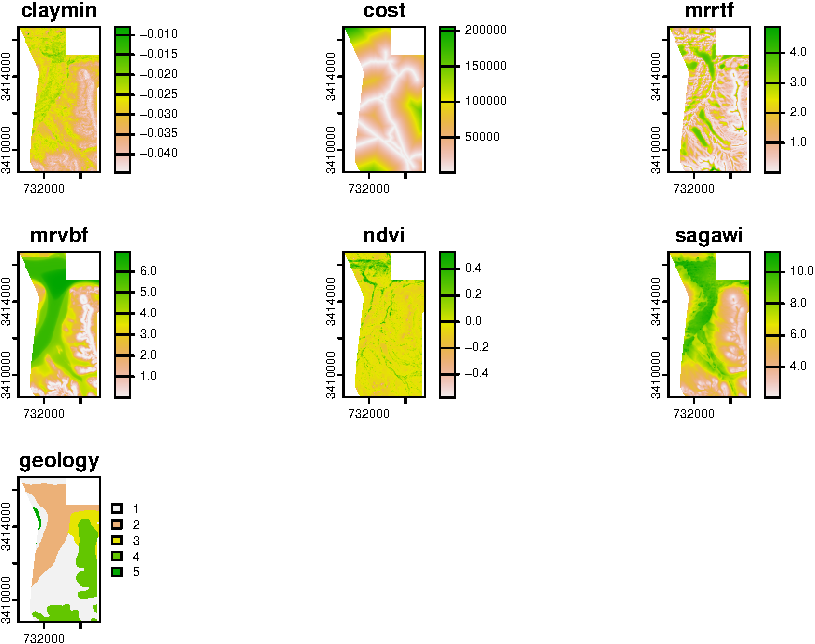
\includegraphics{Technical-Manual-Soil-Sampling-Design_files/figure-latex/fig-15-1.pdf}
\caption{\label{fig:fig-15}Covariates}
\end{figure}

The distribution of the sampling points is obtained using the \texttt{\textquotesingle{}cLHS\textquotesingle{}}function together with the stack of raster covariates and the minimum number of samples calculated in the previous Section. The function uses a number of iterations for the Metropolis--Hastings annealing process, with a default of 10000, to determine the optimal location of samples that account for a maximum of information on the raster covariates (Fig. \ref{fig:fig-16}. .

\begin{Shaded}
\begin{Highlighting}[]
  \CommentTok{\# Distribute sampling points with clhs}
\NormalTok{  pts }\OtherTok{\textless{}{-}} \FunctionTok{clhs}\NormalTok{(cov.dat.ras, }\AttributeTok{size =}\NormalTok{ minimum\_n, }\AttributeTok{iter =} \DecValTok{5000}\NormalTok{, }\AttributeTok{progress =} \ConstantTok{FALSE}\NormalTok{, }\AttributeTok{simple =} \ConstantTok{FALSE}\NormalTok{)}
  \CommentTok{\# Plot of objective function}
  \FunctionTok{plot}\NormalTok{(pts, }\FunctionTok{c}\NormalTok{(}\StringTok{\textquotesingle{}obj\textquotesingle{}}\NormalTok{))}
\end{Highlighting}
\end{Shaded}

\begin{figure}
\centering
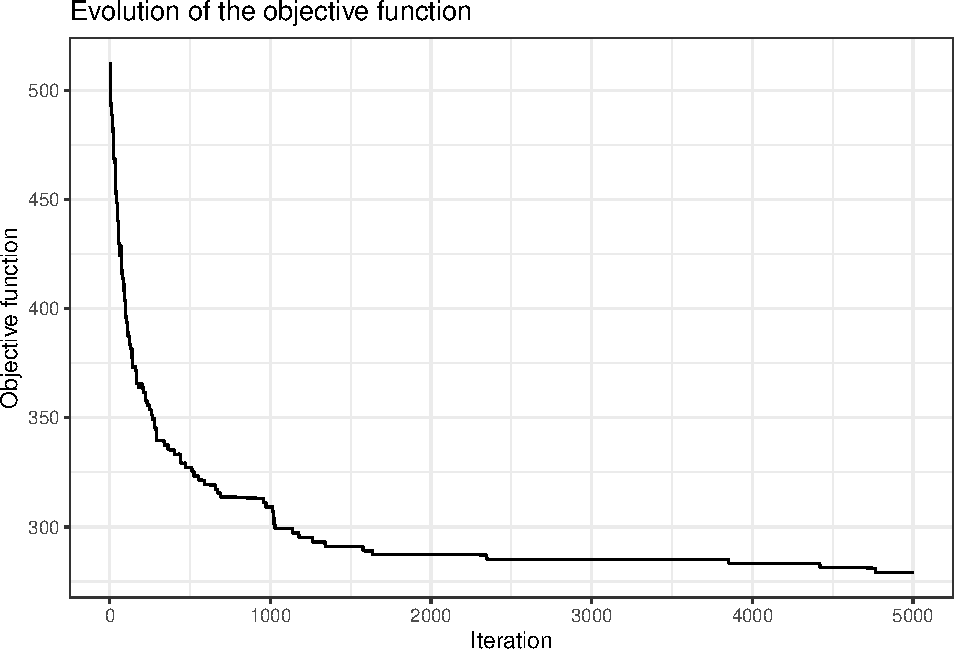
\includegraphics{Technical-Manual-Soil-Sampling-Design_files/figure-latex/fig-16-1.pdf}
\caption{\label{fig:fig-16}Evolution of the objective function}
\end{figure}

The distribution of points is shown in Figure \ref{fig:fig-17}.

\begin{Shaded}
\begin{Highlighting}[]
  \DocumentationTok{\#\# Create a cLHS sampling point set{-}{-}{-}{-}}
    \FunctionTok{plot}\NormalTok{(cov.dat[[}\DecValTok{1}\NormalTok{]], }\AttributeTok{main=}\StringTok{"cLHS samples"}\NormalTok{)}
    \FunctionTok{points}\NormalTok{(pts}\SpecialCharTok{$}\NormalTok{sampled\_data, }\AttributeTok{col=}\StringTok{"red"}\NormalTok{, }\AttributeTok{pch =} \DecValTok{1}\NormalTok{)}
\end{Highlighting}
\end{Shaded}

\begin{figure}
\centering
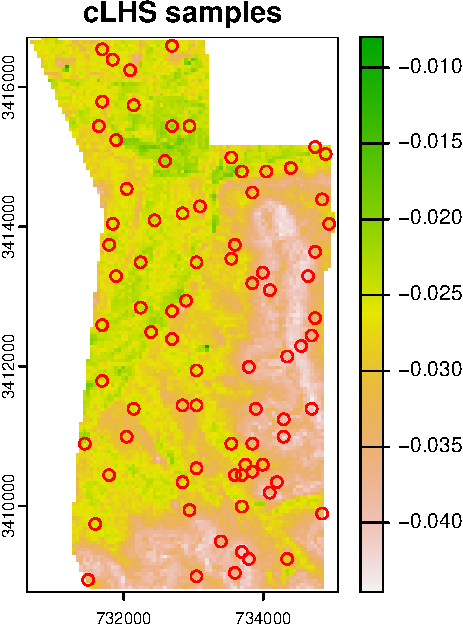
\includegraphics{Technical-Manual-Soil-Sampling-Design_files/figure-latex/fig-17-1.pdf}
\caption{\label{fig:fig-17}Distribution of cLHS sampling points in the study area}
\end{figure}

\hypertarget{including-existing-legacy-data-in-a-chls-sampling-design}{%
\section{Including existing legacy data in a cHLS sampling design}\label{including-existing-legacy-data-in-a-chls-sampling-design}}

In situations where there are legacy soil data samples available, it would be interesting to include them in the cLHS design to increase the diversity of covariates and avoid oversampling for some conditions. In this cases, the ancillary data can be included in the design as additional points to the \texttt{\textquotesingle{}clhs\textquotesingle{}} function.

\begin{Shaded}
\begin{Highlighting}[]
\CommentTok{\# We create an artificial legacy dataset of 20 samples over the study area}
\NormalTok{  legacy.data }\OtherTok{\textless{}{-}} \FunctionTok{spatSample}\NormalTok{(cov.dat,}\DecValTok{20}\NormalTok{, }\AttributeTok{na.rm=}\ConstantTok{TRUE}\NormalTok{,}\AttributeTok{xy=}\ConstantTok{TRUE}\NormalTok{,}\AttributeTok{method=}\StringTok{"random"}\NormalTok{, }\AttributeTok{as.points=}\NormalTok{T) }\CommentTok{\# works with SpatRaster }

  \CommentTok{\# Get covariates data as a points}
\NormalTok{  cov.df}\OtherTok{\textless{}{-}} \FunctionTok{as.points}\NormalTok{(cov.dat)}
  
\CommentTok{\# Merge legacy and covariate information}
\NormalTok{  leg.new }\OtherTok{\textless{}{-}}   \FunctionTok{rbind}\NormalTok{(legacy.data, cov.df)}
\NormalTok{  leg.new }\OtherTok{\textless{}{-}} \FunctionTok{as.data.frame}\NormalTok{(leg.new,}\AttributeTok{geom=}\StringTok{\textquotesingle{}XY\textquotesingle{}}\NormalTok{)}
  \CommentTok{\# Delete data from pixels outside the study area}
\NormalTok{  leg.new }\OtherTok{\textless{}{-}} \FunctionTok{na.omit}\NormalTok{(leg.new)}
  
\CommentTok{\# Calculate clhs 100 points plus locations of legacy data}
\NormalTok{    res }\OtherTok{\textless{}{-}} \FunctionTok{clhs}\NormalTok{(}\AttributeTok{x =}\NormalTok{ leg.new, }\AttributeTok{size =} \DecValTok{100}\SpecialCharTok{+}\FunctionTok{length}\NormalTok{(legacy.data),  }\AttributeTok{iter =} \DecValTok{10000}\NormalTok{,}\AttributeTok{simple =} \ConstantTok{FALSE}\NormalTok{, }\AttributeTok{progress =} \ConstantTok{FALSE}\NormalTok{,}
            \AttributeTok{must.include =} \FunctionTok{c}\NormalTok{(}\DecValTok{1}\SpecialCharTok{:}\FunctionTok{nrow}\NormalTok{(legacy.data)))}

\CommentTok{\# Get sampling points}
\NormalTok{  points }\OtherTok{\textless{}{-}}\NormalTok{ res}\SpecialCharTok{$}\NormalTok{sampled\_data}
\end{Highlighting}
\end{Shaded}

Figure \ref{fig:fig-18} shows the distribution of the created cLHS samples, which also include the position of the original legacy soil data points.

\begin{Shaded}
\begin{Highlighting}[]
\CommentTok{\# Plot points}
  \FunctionTok{plot}\NormalTok{(cov.dat[[}\DecValTok{1}\NormalTok{]], }\AttributeTok{main=}\StringTok{"cLHS samples (blue circles) and legacy samples (red diamonds)"}\NormalTok{)}
  \FunctionTok{points}\NormalTok{(points[,}\FunctionTok{c}\NormalTok{(}\StringTok{"x"}\NormalTok{,}\StringTok{"y"}\NormalTok{)], }\AttributeTok{col=}\StringTok{"dodgerblue"}\NormalTok{, }\AttributeTok{pch =} \DecValTok{1}\NormalTok{)}
  \FunctionTok{points}\NormalTok{(legacy.data, }\AttributeTok{col=}\StringTok{"red"}\NormalTok{, }\AttributeTok{pch =} \DecValTok{5}\NormalTok{, }\AttributeTok{cex=}\DecValTok{2}\NormalTok{)}
\end{Highlighting}
\end{Shaded}

\begin{figure}
\centering
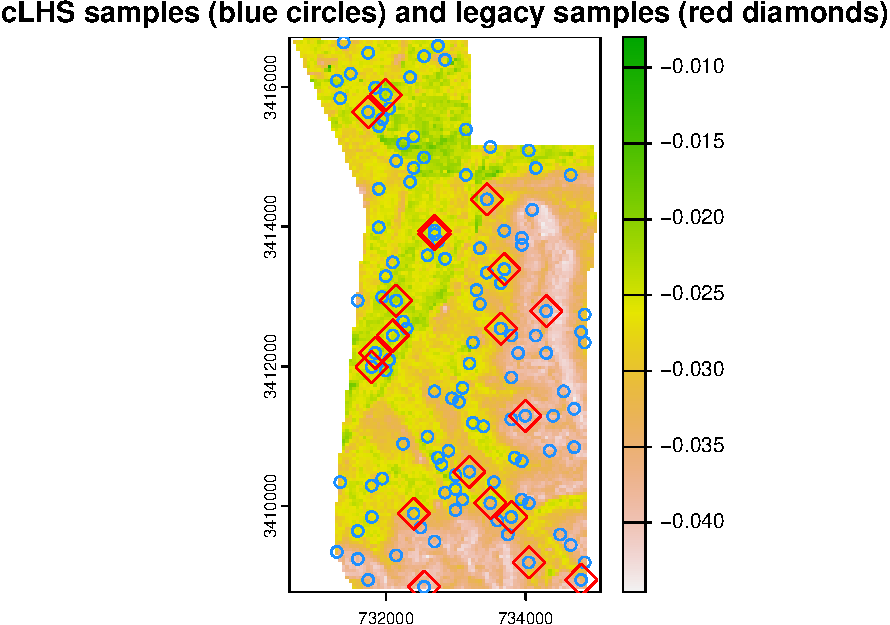
\includegraphics{Technical-Manual-Soil-Sampling-Design_files/figure-latex/fig-18-1.pdf}
\caption{\label{fig:fig-18}cLHS sampling points with legacy data}
\end{figure}

\hypertarget{working-with-large-raster-data}{%
\section{Working with large raster data}\label{working-with-large-raster-data}}

The cLHS function samples the covariates in the raster stack in order to determine the optimal location of samples that best represent the environmental conditions in the area. In the case of working with large raster sets, the process can be highly computing demanding since all pixels in the raster stack are used in the process. There are two simple methods to avoid this constraint:

\begin{itemize}
\tightlist
\item
  \textbf{Aggregation of covariates:} The quickest solution is to aggregate the covariates in the raster stack to a lower pixel resolution. This is directly performed using the \texttt{\textquotesingle{}aggregate\textquotesingle{}} function from the \texttt{\textquotesingle{}terra\textquotesingle{}}package. In case that the raster stack has discrete layers (factor data), the corresponding layers has to be aggregated separately using either the `min' or `max' functions to avoid corruption of the data and the results added later to the data of continuous raster layers.
\end{itemize}

\begin{Shaded}
\begin{Highlighting}[]
  \DocumentationTok{\#\# Aggregation of raster stack by a factor of 2. }
  \DocumentationTok{\#\# The original 10x10m grid resolution is resampled to 20x20m using the mean value of the pixels in the grid}
\NormalTok{    cov.dat }\OtherTok{\textless{}{-}} \FunctionTok{aggregate}\NormalTok{(cov.dat, }\AttributeTok{fact=}\DecValTok{2}\NormalTok{, }\AttributeTok{fun=}\StringTok{"mean"}\NormalTok{)}
\end{Highlighting}
\end{Shaded}

\begin{itemize}
\tightlist
\item
  \textbf{Sampling covariate data:} Other method that can be used is to sample the stack (extract the covariates information at point scale) on a regular grid at a lower resolution than the raster grid and use this information as input within the cLHS function. The creation of a regular point grid on the raster stack is straightforward through the function \texttt{spatSample} from the \texttt{\textquotesingle{}terra\textquotesingle{}} package. In this case we create a regular grid of 1000 points.
\end{itemize}

\begin{Shaded}
\begin{Highlighting}[]
  \CommentTok{\# Create a regular grid of 1000 points on the covariate space}
\NormalTok{    regular.sample }\OtherTok{\textless{}{-}} \FunctionTok{spatSample}\NormalTok{(cov.dat, }\AttributeTok{size =} \DecValTok{1000}\NormalTok{, }\AttributeTok{xy=}\ConstantTok{TRUE}\NormalTok{, }\AttributeTok{method=}\StringTok{"regular"}\NormalTok{, }\AttributeTok{na.rm=}\ConstantTok{TRUE}\NormalTok{)}
  \CommentTok{\# plot the points over the 1st raster}
    \FunctionTok{plot}\NormalTok{(cov.dat[[}\DecValTok{1}\NormalTok{]], }\AttributeTok{main=}\StringTok{"Regular resampled data"}\NormalTok{)}
    \FunctionTok{points}\NormalTok{(regular.sample, }\AttributeTok{col=}\StringTok{"red"}\NormalTok{, }\AttributeTok{pch =} \DecValTok{1}\NormalTok{)}
\end{Highlighting}
\end{Shaded}

\begin{figure}
\centering
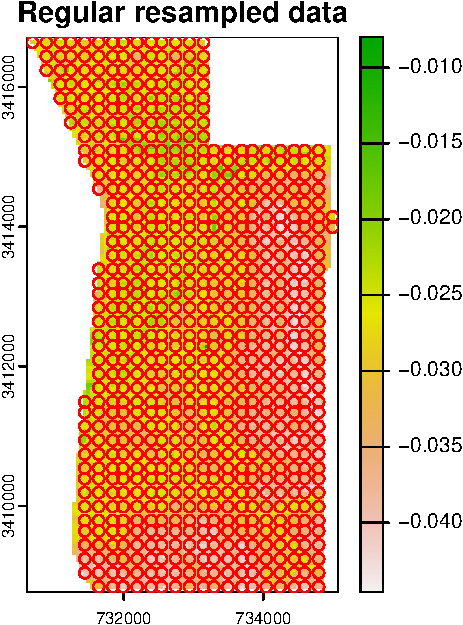
\includegraphics{Technical-Manual-Soil-Sampling-Design_files/figure-latex/fig-19-1.pdf}
\caption{\label{fig:fig-19}Low resolution points of covariate data}
\end{figure}

This \texttt{dataframe} can be directly used as input in the cLHS function to get locations that best represent the covariate space in the area.

\begin{Shaded}
\begin{Highlighting}[]
  \CommentTok{\# Create clhs samples upon the regular grid  }
\NormalTok{   regular.sample.clhs }\OtherTok{\textless{}{-}} \FunctionTok{clhs}\NormalTok{(regular.sample, }\AttributeTok{size =} \DecValTok{100}\NormalTok{, }\AttributeTok{progress =} \ConstantTok{FALSE}\NormalTok{, }\AttributeTok{iter =} \DecValTok{10000}\NormalTok{, }\AttributeTok{simple =} \ConstantTok{FALSE}\NormalTok{)}
  \CommentTok{\# Plot points of clhs samples}
\NormalTok{    points }\OtherTok{\textless{}{-}}\NormalTok{ regular.sample.clhs}\SpecialCharTok{$}\NormalTok{sampled\_data }\CommentTok{\# Get point coordinates of clhs sampling}
    \FunctionTok{plot}\NormalTok{(cov.dat[[}\DecValTok{1}\NormalTok{]], }\AttributeTok{main=}\StringTok{"cLHS samples (red) and covariated resampled points (blue)"}\NormalTok{)}
    \FunctionTok{points}\NormalTok{(regular.sample, }\AttributeTok{col=}\StringTok{"dodgerblue"}\NormalTok{, }\AttributeTok{pch =} \DecValTok{1}\NormalTok{)}
    \FunctionTok{points}\NormalTok{(points, }\AttributeTok{col=}\StringTok{"red"}\NormalTok{, }\AttributeTok{cex=}\DecValTok{1}\NormalTok{)}
\end{Highlighting}
\end{Shaded}

\begin{figure}
\centering
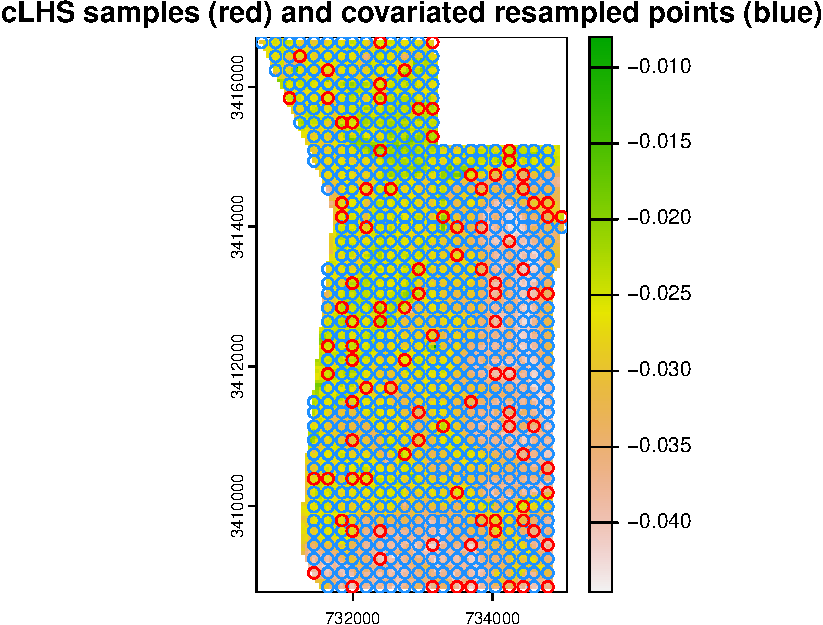
\includegraphics{Technical-Manual-Soil-Sampling-Design_files/figure-latex/fig-20-1.pdf}
\caption{\label{fig:fig-20}cLHS sampling points on point-grid transformed raster covariate data}
\end{figure}

Note that the sampling design follows the regular pattern of the regular grid extracted from the raster covariates

\hypertarget{implemenentation-of-costconstrained-sampling}{%
\section{Implemenentation of cost--constrained sampling}\label{implemenentation-of-costconstrained-sampling}}

There are situation in which the accessibility to some locations is totally or partially restricted such as areas with steep slopes, remote areas, or areas with forbidden access, which highly compromises the sampling process. For these cases, the sampling design can constrain the points to particular locations by defining environmental layers that cause an increment in the cost efficiency of the sampling. This is done with the \texttt{cost} attribute in the main \texttt{\textquotesingle{}clhs\textquotesingle{}} function. The following example uses the raster layer ``distance to roads'' as a cost layer to avoid low accessible points located at large distance from roads while optimizing the representativeness of the remaining environmental covariates.

\begin{Shaded}
\begin{Highlighting}[]
  \CommentTok{\# Create a cLHS sampling point set with }
\NormalTok{  cost.clhs }\OtherTok{\textless{}{-}} \FunctionTok{clhs}\NormalTok{(cov.dat.ras, }\AttributeTok{size =}\NormalTok{ minimum\_n, }\AttributeTok{iter =} \DecValTok{5000}\NormalTok{, }\AttributeTok{progress =} \ConstantTok{FALSE}\NormalTok{, }\AttributeTok{simple =} \ConstantTok{FALSE}\NormalTok{, }\AttributeTok{cost =} \StringTok{\textquotesingle{}cost\textquotesingle{}}\NormalTok{,  }\AttributeTok{use.cpp =}\NormalTok{ T)}
  \CommentTok{\# Plot objective function}
  \FunctionTok{plot}\NormalTok{(pts, }\FunctionTok{c}\NormalTok{(}\StringTok{\textquotesingle{}obj\textquotesingle{}}\NormalTok{, }\StringTok{\textquotesingle{}cost\textquotesingle{}}\NormalTok{))}
\end{Highlighting}
\end{Shaded}

\begin{figure}
\centering
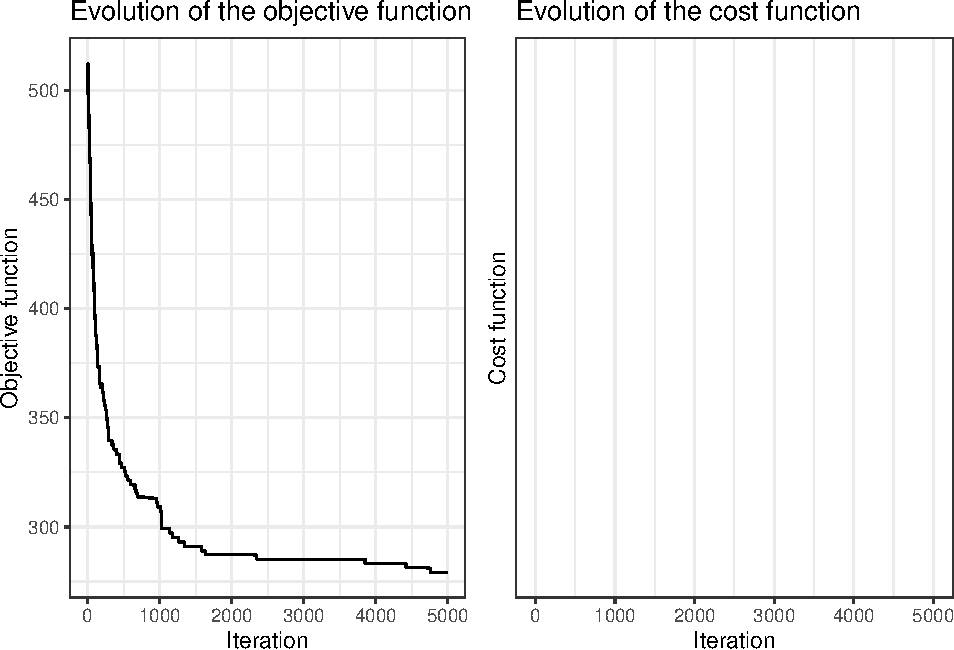
\includegraphics{Technical-Manual-Soil-Sampling-Design_files/figure-latex/fig-21-1.pdf}
\caption{\label{fig:fig-21}Objective and cost funtions}
\end{figure}

Figure \ref{fig:fig-22} shows the distribution of the cost constrained \texttt{\textquotesingle{}clhs\textquotesingle{}} sampling over the \texttt{\textquotesingle{}cost\textquotesingle{}} surface. The sampling procedure concentrates, as much as possible, sampling sites in locations with lower costs.

\begin{Shaded}
\begin{Highlighting}[]
  \CommentTok{\# Get and plot the point of samples}
\NormalTok{  points }\OtherTok{\textless{}{-}}\NormalTok{ cost.clhs}\SpecialCharTok{$}\NormalTok{sampled\_data  }\CommentTok{\# Get point coordinates of clhs sampling}
  \FunctionTok{plot}\NormalTok{(cov.dat[[}\DecValTok{2}\NormalTok{]], }\AttributeTok{main=}\StringTok{"cLHS samples with \textquotesingle{}cost\textquotesingle{} constraints"}\NormalTok{)}
  \FunctionTok{points}\NormalTok{(points, }\AttributeTok{col=}\StringTok{"red"}\NormalTok{, }\AttributeTok{cex=}\DecValTok{1}\NormalTok{)}
\end{Highlighting}
\end{Shaded}

\begin{figure}
\centering
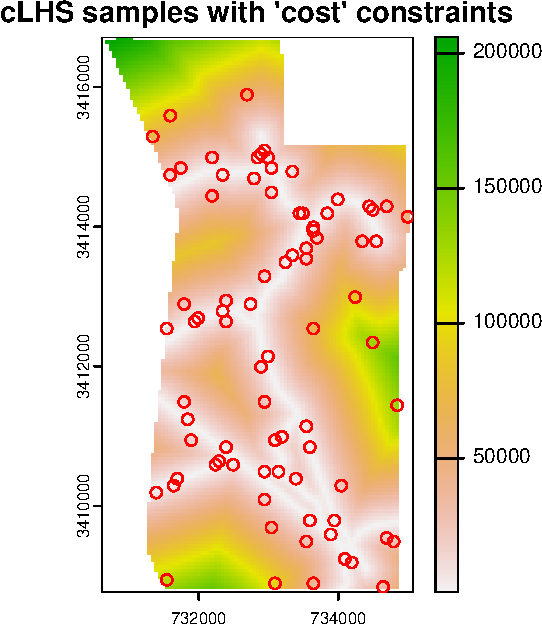
\includegraphics{Technical-Manual-Soil-Sampling-Design_files/figure-latex/fig-22-1.pdf}
\caption{\label{fig:fig-22}cLHS sampling with cost layers}
\end{figure}

Cost surfaces can be defined by other parameters than distances to roads. They can represent private property boundaries, slopes, presence of wetlands, etc. The package \texttt{\textquotesingle{}sgsR\textquotesingle{}} implements functions to define both cost surfaces and distances to roads simultaneously. In this case, it is possible to define an inner buffer distance -- i.e.~the distance from the roads that should be avoided for sampling and an outer buffer -- i.e.~the maximum sampling distance) from roads to maximize the variability of the sampling point while considering these limits. The \texttt{\textquotesingle{}sample\_clhs\textquotesingle{}} function in this package also includes options to include existing legacy data in the process of clhs sampling.

\begin{Shaded}
\begin{Highlighting}[]
\CommentTok{\# Load, roads and legacy data }
\NormalTok{  roads }\OtherTok{\textless{}{-}}\NormalTok{ sf}\SpecialCharTok{::}\FunctionTok{st\_read}\NormalTok{(}\FunctionTok{file.path}\NormalTok{(}\FunctionTok{paste0}\NormalTok{(shp.path,}\StringTok{"/road.shp"}\NormalTok{)),}\AttributeTok{quiet=}\ConstantTok{TRUE}\NormalTok{)}
\NormalTok{  legacy }\OtherTok{\textless{}{-}}\NormalTok{ sf}\SpecialCharTok{::}\FunctionTok{st\_read}\NormalTok{(}\FunctionTok{file.path}\NormalTok{(}\FunctionTok{paste0}\NormalTok{(shp.path,}\StringTok{"/legacy\_soils.shp"}\NormalTok{)),}\AttributeTok{quiet=}\ConstantTok{TRUE}\NormalTok{)}

  \CommentTok{\# Calculate distance to roads and delete NA in outputs}
\NormalTok{  cost }\OtherTok{\textless{}{-}}\NormalTok{ cov.dat }
\NormalTok{  dist2access }\OtherTok{\textless{}{-}}\NormalTok{ terra}\SpecialCharTok{::}\FunctionTok{distance}\NormalTok{(cov.dat[[}\DecValTok{1}\NormalTok{]], roads, }\AttributeTok{progress=}\NormalTok{F)}
\NormalTok{  cost}\SpecialCharTok{$}\NormalTok{dist2access}\OtherTok{\textless{}{-}}\NormalTok{ dist2access}\SpecialCharTok{*}\NormalTok{cost}\SpecialCharTok{$}\NormalTok{claymin}\SpecialCharTok{/}\NormalTok{cost}\SpecialCharTok{$}\NormalTok{claymin}

\CommentTok{\# Calculate clhs points with legacy, cost and buffer to roads}
\NormalTok{  buff\_inner}\OtherTok{=}\DecValTok{20}\NormalTok{;}
\NormalTok{  buff\_outer}\OtherTok{=}\DecValTok{300}
\NormalTok{  aa }\OtherTok{\textless{}{-}} \FunctionTok{sample\_clhs}\NormalTok{(}\AttributeTok{mraster =}\NormalTok{ cost, }\AttributeTok{nSamp =} \DecValTok{300}\NormalTok{, }\AttributeTok{existing =}\NormalTok{ legacy, }\AttributeTok{iter =} \DecValTok{250}\NormalTok{, }\AttributeTok{details =} \ConstantTok{TRUE}\NormalTok{, }\AttributeTok{cost=}\StringTok{"cost"}\NormalTok{, }\AttributeTok{access=}\NormalTok{roads, }\AttributeTok{buff\_inner=}\NormalTok{buff\_inner, }\AttributeTok{buff\_outer=}\NormalTok{buff\_outer)}
\end{Highlighting}
\end{Shaded}

\begin{Shaded}
\begin{Highlighting}[]
\DocumentationTok{\#\# Plot distances, roads, clhs points and legacy data }
  \FunctionTok{plot}\NormalTok{(cost}\SpecialCharTok{$}\NormalTok{dist2access)}
  \FunctionTok{plot}\NormalTok{(roads,}\AttributeTok{add=}\ConstantTok{TRUE}\NormalTok{)}
  \FunctionTok{plot}\NormalTok{(aa}\SpecialCharTok{$}\NormalTok{samples[aa}\SpecialCharTok{$}\NormalTok{samples}\SpecialCharTok{$}\NormalTok{type}\SpecialCharTok{==}\StringTok{"new"}\NormalTok{,], }\AttributeTok{col=} \StringTok{"tomato"}\NormalTok{,}\AttributeTok{add=}\ConstantTok{TRUE}\NormalTok{)}
  \FunctionTok{plot}\NormalTok{(aa}\SpecialCharTok{$}\NormalTok{samples[aa}\SpecialCharTok{$}\NormalTok{samples}\SpecialCharTok{$}\NormalTok{type}\SpecialCharTok{==}\StringTok{"existing"}\NormalTok{,], }\AttributeTok{col=} \StringTok{"navy"}\NormalTok{,}\AttributeTok{add=}\ConstantTok{TRUE}\NormalTok{)}
\end{Highlighting}
\end{Shaded}

\begin{figure}
\centering
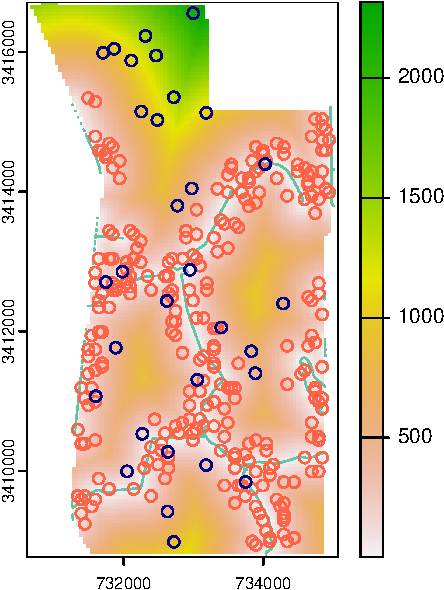
\includegraphics{Technical-Manual-Soil-Sampling-Design_files/figure-latex/fig-22b-1.pdf}
\caption{\label{fig:fig-22b}cLHS sampling with legacy data, cost surface and distance buffers around roads}
\end{figure}

Legacy data is represented as blue dots while new samples from cLHS analyses are in red colour (Fig.\ref{fig:fig-22}). Note that the new sampling points are located within a distance buffer of 20-300 meters from roads. In addition, a cost surface has also been included in the analyses.

\hypertarget{replacement-areas-in-clhs-design}{%
\section{Replacement areas in cLHS design}\label{replacement-areas-in-clhs-design}}

The \texttt{\textquotesingle{}cLHS\textquotesingle{}} package incorporates methods for the delineation of replacement locations that could be utilized in the case any sampling point is unreachable. In this case, the function determines the probability of similarity to each point in an area determined by a buffer distance around the points.

\begin{Shaded}
\begin{Highlighting}[]
  \DocumentationTok{\#\# Determine the similarity to points in a buffer of distance D}
  \CommentTok{\# Compute the buffers around points  }
\NormalTok{    gw }\OtherTok{\textless{}{-}} \FunctionTok{similarity\_buffer}\NormalTok{(cov.dat.ras, pts}\SpecialCharTok{$}\NormalTok{sampled\_data, }\AttributeTok{buffer =}\NormalTok{ D)}
\end{Highlighting}
\end{Shaded}

The similarity probabilities for the first cLHS point is presented on Figure \ref{fig:fig-23} over the elevation layer.

\begin{Shaded}
\begin{Highlighting}[]
  \CommentTok{\# Plot elevation}
    \FunctionTok{plot}\NormalTok{(cov.dat[[}\DecValTok{3}\NormalTok{]], }\AttributeTok{legend=}\ConstantTok{TRUE}\NormalTok{,}\AttributeTok{main=}\FunctionTok{paste}\NormalTok{(}\StringTok{"Similarity Probability over elevation"}\NormalTok{))}
  \DocumentationTok{\#\# Overlay points}
    \FunctionTok{points}\NormalTok{(pts}\SpecialCharTok{$}\NormalTok{sampled\_data[}\DecValTok{1}\NormalTok{], }\AttributeTok{col =} \StringTok{"dodgerblue"}\NormalTok{, }\AttributeTok{pch =} \DecValTok{3}\NormalTok{)}
  \DocumentationTok{\#\# Overlay probability stack for point 1}
\NormalTok{    colors }\OtherTok{\textless{}{-}} \FunctionTok{c}\NormalTok{((RColorBrewer}\SpecialCharTok{::}\FunctionTok{brewer.pal}\NormalTok{(}\DecValTok{9}\NormalTok{, }\StringTok{"YlOrRd"}\NormalTok{)))}
\NormalTok{    terra}\SpecialCharTok{::}\FunctionTok{plot}\NormalTok{(gw[[}\DecValTok{1}\NormalTok{]], }\AttributeTok{add=}\ConstantTok{TRUE}\NormalTok{ ,  }\AttributeTok{legend=}\ConstantTok{FALSE}\NormalTok{, }\AttributeTok{col=}\NormalTok{colors)}
  \DocumentationTok{\#\# Overlay 1st cLHS point}
    \FunctionTok{points}\NormalTok{(pts}\SpecialCharTok{$}\NormalTok{sampled\_data[}\DecValTok{1}\NormalTok{,}\DecValTok{1}\NormalTok{], }\AttributeTok{col =} \StringTok{"black"}\NormalTok{, }\AttributeTok{pch =} \DecValTok{3}\NormalTok{,}\AttributeTok{cex=}\DecValTok{1}\NormalTok{)}
\end{Highlighting}
\end{Shaded}

\begin{figure}
\centering
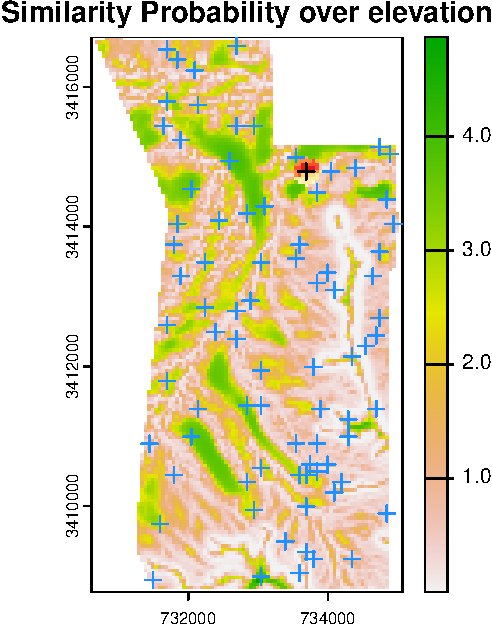
\includegraphics{Technical-Manual-Soil-Sampling-Design_files/figure-latex/fig-23-1.pdf}
\caption{\label{fig:fig-23}Probability of similarity in the buffer for the first cLHS point (in black) over elevation. The blue crosses represent the location of the remaining cLHS points from the analysis.}
\end{figure}

The probabilities can then be reclassified using a threshold value to delineate the areas with higher similarity to each central target point.

\begin{Shaded}
\begin{Highlighting}[]
  \CommentTok{\# Determine the threshold break to determine if the surrounding area can be a replacement or not}
\NormalTok{    similarity\_threshold }\OtherTok{\textless{}{-}} \FloatTok{0.90}
  \CommentTok{\# Reclassify buffer raster data according to the threshold break of probability}
  \CommentTok{\# 1 = similarity \textgreater{}= similarity\_break; NA =  similarity \textless{}  similarity\_break}
    \CommentTok{\# Define a vector with the break intervals and the output values (NA,1) }
\NormalTok{    breaks }\OtherTok{\textless{}{-}} \FunctionTok{c}\NormalTok{(}\DecValTok{0}\NormalTok{, similarity\_threshold, }\ConstantTok{NA}\NormalTok{, similarity\_threshold, }\DecValTok{1}\NormalTok{, }\DecValTok{1}\NormalTok{)}
    \CommentTok{\# Convert to a matrix}
\NormalTok{    breaks }\OtherTok{\textless{}{-}} \FunctionTok{matrix}\NormalTok{(breaks, }\AttributeTok{ncol=}\DecValTok{3}\NormalTok{, }\AttributeTok{byrow=}\ConstantTok{TRUE}\NormalTok{)}
    \CommentTok{\# Reclassify the data in the layers from probabilities to (NA,)}
\NormalTok{    s }\OtherTok{=} \FunctionTok{stack}\NormalTok{(}\FunctionTok{lapply}\NormalTok{(}\DecValTok{1}\SpecialCharTok{:}\NormalTok{raster}\SpecialCharTok{::}\FunctionTok{nlayers}\NormalTok{(gw), }\ControlFlowTok{function}\NormalTok{(i)\{raster}\SpecialCharTok{::}\FunctionTok{reclassify}\NormalTok{(gw[[i]], breaks, }\AttributeTok{right=}\ConstantTok{FALSE}\NormalTok{)\}))}
\end{Highlighting}
\end{Shaded}

The reclassified raster stack is then converted to an object of \texttt{\textquotesingle{}SpatialPolygonsDataFrame\textquotesingle{}} class.

\begin{Shaded}
\begin{Highlighting}[]
   \DocumentationTok{\#\# Polygonize replacement areas }
\NormalTok{    s }\OtherTok{=} \FunctionTok{lapply}\NormalTok{(}\FunctionTok{as.list}\NormalTok{(s), rasterToPolygons, }\AttributeTok{dissolve=}\ConstantTok{TRUE}\NormalTok{)}
\NormalTok{    s }\OtherTok{\textless{}{-}} \FunctionTok{bind}\NormalTok{(s,}\AttributeTok{keepnames=}\ConstantTok{TRUE}\NormalTok{)}
    
    \CommentTok{\# Add the identifier of the corresponding target point}
    \ControlFlowTok{for}\NormalTok{(i }\ControlFlowTok{in} \DecValTok{1}\SpecialCharTok{:} \FunctionTok{length}\NormalTok{(s))\{}
\NormalTok{      s}\SpecialCharTok{@}\NormalTok{data}\SpecialCharTok{$}\NormalTok{ID[i] }\OtherTok{\textless{}{-}} \FunctionTok{as.integer}\NormalTok{(stringr}\SpecialCharTok{::}\FunctionTok{str\_replace}\NormalTok{(s}\SpecialCharTok{@}\NormalTok{polygons[[i]]}\SpecialCharTok{@}\NormalTok{ID,}\StringTok{"1."}\NormalTok{,}\StringTok{""}\NormalTok{))}
\NormalTok{    \}}
    \CommentTok{\# Clean the data by storing target ID data only}
\NormalTok{    s}\SpecialCharTok{@}\NormalTok{data }\OtherTok{\textless{}{-}}\NormalTok{ s}\SpecialCharTok{@}\NormalTok{data[}\StringTok{"ID"}\NormalTok{]}
\end{Highlighting}
\end{Shaded}

The results are shown in Figure \ref{fig:fig-24}.

\begin{Shaded}
\begin{Highlighting}[]
    \FunctionTok{plot}\NormalTok{(cov.dat[[}\DecValTok{1}\NormalTok{]], }\AttributeTok{main=}\FunctionTok{paste}\NormalTok{(}\StringTok{"cLHS samples and replacement areas for threshold = "}\NormalTok{, similarity\_threshold))}
    \FunctionTok{plot}\NormalTok{(s,}\AttributeTok{add=}\ConstantTok{TRUE}\NormalTok{, }\AttributeTok{col=}\ConstantTok{NA}\NormalTok{, }\AttributeTok{border=}\StringTok{"gray40"}\NormalTok{)}
    \FunctionTok{points}\NormalTok{(pts}\SpecialCharTok{$}\NormalTok{sampled\_data, }\AttributeTok{col=}\StringTok{"red"}\NormalTok{, }\AttributeTok{pch =} \DecValTok{3}\NormalTok{)}
\end{Highlighting}
\end{Shaded}

\begin{figure}
\centering
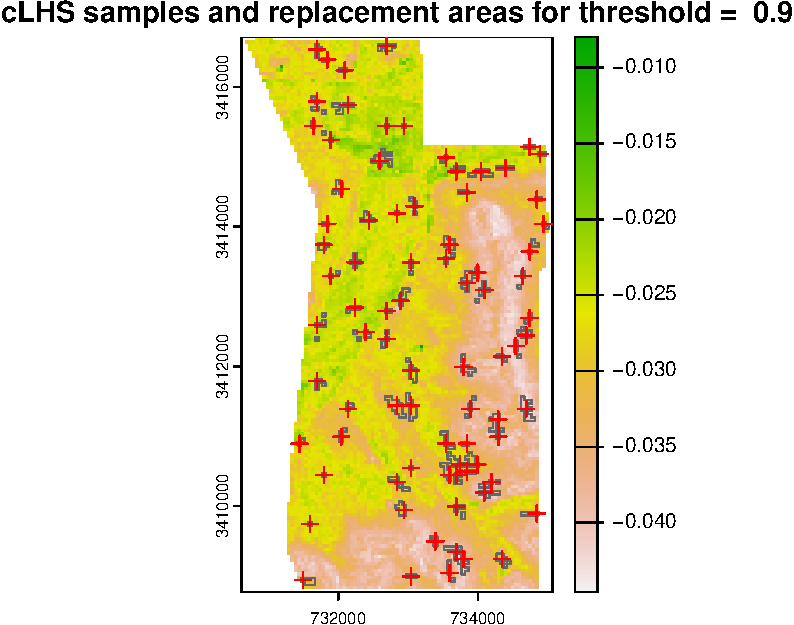
\includegraphics{Technical-Manual-Soil-Sampling-Design_files/figure-latex/fig-24-1.pdf}
\caption{\label{fig:fig-24}Distribution of cLHS sampling points in the study area}
\end{figure}

The layer of replacement areas can finally be exported to a \texttt{\textquotesingle{}shapefile\textquotesingle{}} to be used in any other software.

\begin{Shaded}
\begin{Highlighting}[]
   \CommentTok{\# Write replacement areas to polygon shape }
\NormalTok{    s }\OtherTok{\textless{}{-}} \FunctionTok{st\_as\_sf}\NormalTok{(s)}
    \FunctionTok{st\_write}\NormalTok{(s, }\FunctionTok{file.path}\NormalTok{(}\FunctionTok{paste0}\NormalTok{(results.path,}\StringTok{\textquotesingle{}replacement\_areas\_\textquotesingle{}}\NormalTok{, D, }\StringTok{\textquotesingle{}.shp\textquotesingle{}}\NormalTok{)), }\AttributeTok{delete\_dsn =} \ConstantTok{TRUE}\NormalTok{)}
  \CommentTok{\# Write cLHS sampling points to shapefile}
\NormalTok{    out.pts }\OtherTok{\textless{}{-}} \FunctionTok{st\_as\_sf}\NormalTok{(pts}\SpecialCharTok{$}\NormalTok{sampled\_data)}
    \FunctionTok{st\_write}\NormalTok{(out.pts, }\FunctionTok{paste0}\NormalTok{(results.path,}\StringTok{\textquotesingle{}target\_clhs.shp\textquotesingle{}}\NormalTok{), }\AttributeTok{delete\_dsn =} \ConstantTok{TRUE}\NormalTok{)}
\end{Highlighting}
\end{Shaded}

\hypertarget{references}{%
\chapter*{References}\label{references}}
\addcontentsline{toc}{chapter}{References}

\hypertarget{refs}{}
\begin{CSLReferences}{0}{0}
\leavevmode\vadjust pre{\hypertarget{ref-sgsR}{}}%
\textbf{Goodbody, T.R.H., Coops, N.C., Queinnec, M., White, J.C., Tompalski, P., Hudak, A.T., Auty, D., Valbuena, R., LeBoeuf, A., Sinclair, I., McCartney, G., Prieur, J.-F. \& Woods, M.E.} 2023. \emph{\href{https://doi.org/10.1093/forestry/cpac055}{sgsR: A structurally guided sampling toolbox for LiDAR-based forest inventories.}}

\leavevmode\vadjust pre{\hypertarget{ref-Malone}{}}%
\textbf{Malone, B.P., Minansy, B. \& Brungard, C.} 2019. Some methods to improve the utility of conditioned latin hypercube sampling. \emph{PeerJ}, 7: e6451. \url{https://doi.org/10.7717/peerj.6451}

\leavevmode\vadjust pre{\hypertarget{ref-minasny2006}{}}%
\textbf{Minasny, B. \& McBratney, A.} 2006. A conditioned latin hypercube method for sampling in the presence of ancillary information. \emph{Computers \& Geosciences}, 32: 1378--1388. \url{https://doi.org/10.1016/j.cageo.2005.12.009}

\leavevmode\vadjust pre{\hypertarget{ref-Roudier2011}{}}%
\textbf{Roudier, P., Brugnard, C., Beaudette, D., Louis, B., Daust, K. \& Clifford, D.} 2011. \emph{Clhs: A r package for conditioned latin hypercube sampling}. (also available at \url{https://cran.r-project.org/web/packages/clhs/}).

\end{CSLReferences}

\end{document}
